\documentclass[14pt]{extarticle}
\usepackage{fontspec}
\usepackage{polyglossia}
\usepackage{amsmath}
\usepackage{amssymb}
\usepackage{xcolor}
\usepackage{fancyhdr}
\usepackage{graphicx}
\usepackage{listings}
\usepackage[most]{tcolorbox}
% \usepackage{setspace}
\usepackage{pifont}
\usepackage{enumitem}
\usepackage{titlesec}
\usepackage[bottom]{footmisc}
\usepackage{titling}
\usepackage{minted}
\usepackage{etoolbox}
\usepackage{array}
\usepackage{extsizes}
\usepackage{float}
\usepackage{booktabs}
\usepackage{hyperref}
\usepackage[onehalfspacing]{setspace}
\usepackage[a4paper, top=2.7cm, bottom=2.7cm, left=2.5cm, right=2.5cm, headheight=1.5cm, headsep=0.5cm]{geometry}
\usepackage{tikz}

\usetikzlibrary{automata, positioning, arrows.meta, arrows}

\newfontfamily\emoji{Segoe UI Emoji}

\pagestyle{fancy}

\setmainlanguage[numerals=western]{arabic}
\setotherlanguage{english}
% \newfontfamily\arabicfont[Script=Arabic]{Amiri}
\newfontfamily\arabicfont[Script=Arabic]{Calibri}
\newfontfamily\arabicfonttt[Script=Arabic]{Courier New}

\lstset{
  language=[Sharp]C,
  numbers=left,
  stepnumber=1,
  numbersep=8pt,
  frame=single,
  basicstyle=\ttfamily\small,
  keywordstyle=\color{blue},
  stringstyle=\color{red},
  commentstyle=\color{green!50!black}
}

\newif\ifdetailed
\ifdefined\setdetailed
  \setdetailed
\fi

\newif\ifwithsols
\ifdefined\setwithsols
  \setwithsols
\fi

% unified tcolorboxes for articles
\tcbset{colback=white, colframe=black, fonttitle=\bfseries, boxrule=0.8pt}
\newtcolorbox{boxDef}[1][]{colback=blue!5!white,colframe=blue!75!black,
  title={{\emoji📘} تعريف\ifx\\#1\\\else ~#1\fi :}}
\newtcolorbox{boxExercise}[1][]{colback=cyan!5!white,colframe=cyan!70!black,
  title={{\emoji🧩} تمرين\ifx\\#1\\\else ~#1\fi :}}
\newtcolorbox{boxExample}[1][]{colback=yellow!5!white,colframe=orange!90!black,
  title={{\emoji📝} مثال\ifx\\#1\\\else ~#1\fi :}}
\newtcolorbox{boxNote}[1][]{colback=gray!10!white,colframe=black,
  title={{\emoji✨} ملاحظة\ifx\\#1\\\else ~#1\fi :}}
\newtcolorbox{boxAttention}[1][]{colback=magenta!10!white,colframe=magenta!80!black,
  title={{\emoji🔔} تنبيه\ifx\\#1\\\else ~#1\fi :}}
\newtcolorbox{boxWarning}[1][]{colback=red!5!white,colframe=red!75!black,
  title={{\emoji⚡} ملاحظة هامة\ifx\\#1\\\else ~#1\fi :}}
\newtcolorbox{boxSolution}[1][]{colback=green!5!white,colframe=green!60!black,
  title={{\emoji✅} حل\ifx\\#1\\\else ~#1\fi :}}
\newtcolorbox{boxSymbol}[1][]{colback=purple!5!white,colframe=purple!70!black,
  title={{\emoji🔣} رمز\ifx\\#1\\\else ~#1\fi :}}
\newtcolorbox{boxHint}[1][]{colback=teal!5!white,colframe=teal!60!black,
  title={{\emoji💡} تلميح\ifx\\#1\\\else ~#1\fi :}}


\tcbset{simplecode/.style={ colback=gray!5, colframe=black!50, boxrule=0.4pt, arc=2pt, left=4pt,right=4pt,top=4pt,bottom=4pt}}
\newenvironment{boxCode}{\begin{tcolorbox}[simplecode]}{\end{tcolorbox}}

\newcolumntype{C}[1]{>{\centering\arraybackslash}p{#1}}

% redefine spaces after titles
\makeatletter
\renewcommand{\@maketitle}{%
  \begin{center}
    {\huge \bfseries \@title \par}%
    \vskip 0.2em % space between title and author
    {\large \@author \par}%
    % \vskip 0.2em % space between author and date
    % {\normalsize \@date \par}%
  \end{center}
}
\makeatother

\fancyhf{} % clear default
\fancypagestyle{plain}{
  \fancyhf{}
  \fancyhead[L]{مدرسة التسامح الشاملة}
  % \fancyhead[L]{
\includegraphics[height=1cm]{../../../images/logoTasamoh.png}}
  \fancyhead[R]{الأستاذ محمود اغبارية}
  \fancyfoot[C]{\thepage}
}

\fancyhead[L]{مدرسة التسامح الشاملة}
\fancyhead[R]{الأستاذ محمود اغبارية}
\fancyfoot[C]{\thepage}
% \date{\today}

\setcounter{tocdepth}{3} % only section subsection and subsubsection in TOC

\newcommand{\importpdfpage}[2]{%
    \thispagestyle{empty}
    \newgeometry{left=0cm,right=0cm,top=0cm,bottom=0cm}
    \includegraphics[page=#2,width=0.95\paperwidth,height=0.95\paperheight,keepaspectratio]{#1}
    \restoregeometry
}

\newcommand{\insertFullImg}[1]{%
    \noindent
    \makebox[\textwidth][c]{
        \includegraphics[width=0.9\paperwidth,keepaspectratio]{#1}%
    }%
}%

% ----------------------


% \begin{document}

% \maketitle

% % \clearpage  % start TOC on a new page
% % \renewcommand{\contentsname}{جدول المحتويات}
% % \tableofcontents
% % \clearpage

% \part*{part 1} % the * prevents numbering
% \section*{مقدمة}
% \subsection*{مثال رياضي}
% \subsubsection*{مثال فرعي}
% \paragraph*{ paragraph 1}
% \subparagraph*{sub paragraph 1}

% \ifdetailed
% \begin{english}
% \begin{minted}{csharp}
% // C# Example
% \end{minted}
% \end{english}
% \fi

% OLD WAY
% \ifdetailed
% \begin{english}
% \begin{lstlisting}
% // C# Example
% \end{lstlisting}
% \end{english}
% \fi

% % 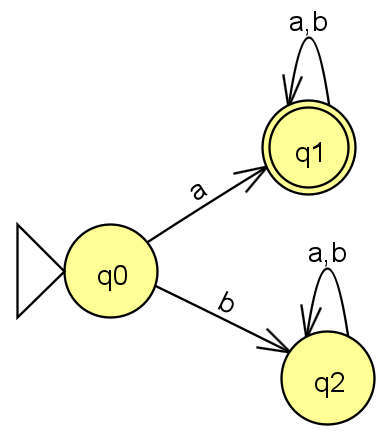
\includegraphics[width=0.2\textwidth]{../../../images/DFAs/ex1_q1.png}



% \vspace{3cm}
% \begin{flushleft}
% أرجو لكم وقتًا ممتعًا.

% الأستاذ محمود اغبارية.
% \end{flushleft}


% \end{document}


\title{آلة تيورينج}

\begin{document}

\maketitle

\renewcommand{\contentsname}{جدول المحتويات}
\tableofcontents
\clearpage

\part{آلة تيورينج (\textenglish{Turing Machine})}

\section{مقدّمة}

\subsection{لماذا نحتاج إلى نموذج جديد؟}

لقد درسنا سابقًا نموذجين حسابيين:
\begin{itemize}
    \item \textbf{الأوتومات النهائي} (\textenglish{Finite Automata - FA}) الذي يتعرف على \textbf{اللغات النظامية} (\textenglish{Regular Languages}).
    \item \textbf{أوتومات الراصّة} (\textenglish{Pushdown Automata - PDA}) الذي يتعرف على \textbf{اللغات خالية السياق} (\textenglish{Context-Free Languages}).
\end{itemize}

لكن، هل هذه النماذج كافية؟

\begin{boxAttention}
هناك لغات بسيطة لا يستطيع أي من النموذجين السابقين التعرف عليها!
\end{boxAttention}

\textbf{مثال:} اللغة $L = \{a^n b^n c^n \mid n \geq 0\}$

هذه اللغة تتكون من كلمات فيها نفس عدد الأحرف $a$ و $b$ و $c$.
\begin{itemize}
    \item كلمات في اللغة: $\varepsilon$, $abc$, $aabbcc$, $aaabbbccc$
    \item كلمات ليست في اللغة: $ab$, $aabbc$, $abcc$
\end{itemize}

\begin{itemize}
    \item الأوتومات النهائي لا يستطيع التعرف عليها لأنه لا يستطيع "عدّ" أو "تذكّر" كميات غير محدودة.
    \item أوتومات الراصّة لا يستطيع التعرف عليها لأنه يحتاج مقارنة \textbf{ثلاثة} أعداد في نفس الوقت، والراصّة تسمح بمقارنة عددين فقط.
\end{itemize}

\textbf{السؤال:} هل يوجد نموذج حسابي أقوى يستطيع التعرف على هذه اللغات؟

\textbf{الجواب:} نعم! \textbf{آلة تيورينج} (\textenglish{Turing Machine})

\clearpage

\subsection{من هو آلن تيورينج؟}

\textbf{آلن ماثيسون تيورينج} (\textenglish{Alan Mathison Turing})\\
(1912-1954)

رياضي بريطاني، من مؤسسي علم الحاسوب. حقق إنجازات استثنائية في الجانب النظري والعملي لعلوم الحاسوب.

\textbf{إنجازاته:}
\begin{itemize}
    \item \textbf{آلة تيورينج:} نموذج مجرد لآلة حاسوب شاملة، يصف طريقة عمل الحاسوب.
    \item \textbf{اختبار تيورينج:} اختبار يفحص ما إذا كان للآلة ذكاء اصطناعي لا يمكن التمييز بينها وبين الإنسان.
\end{itemize}

\begin{boxAttention}
\textbf{فرضية تشرتش-تيورينج} (\textenglish{Church-Turing Thesis}):

كل حساب أو خوارزمية قابلة للتنفيذ، يمكن ترجمتها إلى آلة تيورينج. من هذا المنظور، آلة تيورينج مكافئة لأي حاسوب، ولذلك تُستخدم في علوم الحاسوب كأساس لدراسة قدرات وقيود الحاسوب النظرية.
\end{boxAttention}

اقترح آلن تيورينج هذا النموذج في عام \textbf{1936}، \textbf{قبل} اختراع الحاسوب الحديث، من أجل إنشاء تعريف رياضي دقيق لـ\textbf{خوارزمية} أو "عملية آلية" حسابية.

\clearpage

\section{ما هي آلة تيورينج؟}

\begin{boxDef}[تعريف: آلة تيورينج]
\textbf{آلة تيورينج} هي نموذج مجرد قادر على تنفيذ أي حساب أو خوارزمية يمكن تنفيذها على حاسوب.

عظمة هذه الآلة في \textbf{بساطتها}، ومع ذلك فهي قادرة على تنفيذ أي حساب أو خوارزمية يمكن تنفيذها على حاسوب. وتُعتبر نموذجًا مجردًا لطريقة عمل الحاسوب.
\end{boxDef}

\subsection{ماذا تستطيع آلة تيورينج أن تفعل؟}

\begin{itemize}
    \item التعرف على \textbf{جميع} عائلات اللغات الصورية (بما في ذلك اللغات النظامية واللغات خالية السياق وأكثر)
    \item تنفيذ حسابات على المدخل
    \item عمليات البحث والترتيب على المدخل
    \item تنفيذ أي خوارزمية
\end{itemize}

\begin{boxNote}
آلة تيورينج هي \textbf{الأوتومات الأقوى} لتنفيذ الحسابات.
\end{boxNote}

\clearpage

\section{مكونات آلة تيورينج}

تتكون آلة تيورينج من المكونات التالية:

\subsection{1. شريط الذاكرة (\textenglish{Tape})}

\begin{itemize}
    \item شريط \textbf{لا نهائي} إلى اليمين
    \item \textbf{محدود من اليسار} بالرمز $\vdash$ (رأس الشريط)
    \item مقسّم إلى \textbf{خانات} (\textenglish{Cells})
    \item في كل خانة يمكن كتابة \textbf{حرف واحد}
    \item الخانات الفارغة تحتوي على الرمز $\triangle$ (رمز الفراغ - \textenglish{Blank})
\end{itemize}

\textbf{مثال على شريط:}
\begin{center}
\begin{tikzpicture}[scale=0.8]
    \foreach \i/\content in {0/$\vdash$, 1/a, 2/b, 3/a, 4/a, 5/$\triangle$, 6/$\triangle$, 7/$\triangle$} {
        \draw (\i,0) rectangle +(1,0.8);
        \node at (\i+0.5,0.4) {\content};
    }
    \node at (8.5, 0.4) {$\ldots$};
\end{tikzpicture}
\end{center}

\subsection{2. الأبجدية المدخلة $\Sigma$ (\textenglish{Input Alphabet})}

\begin{itemize}
    \item مجموعة \textbf{نهائية} من أحرف المدخل للغة التي تتعرف عليها الآلة
    \item \textbf{مثال:} $\Sigma = \{a, b\}$
\end{itemize}

\subsection{3. أبجدية الآلة $\Gamma$ (\textenglish{Machine Alphabet})}

\begin{itemize}
    \item مجموعة \textbf{نهائية} من الأحرف التي يمكن كتابتها على الشريط
    \item يحددها \textbf{بانٍ الآلة}
    \item تحتوي على أحرف المدخل $\Sigma \subseteq \Gamma$
    \item تحتوي على رموز مساعدة للعمل الداخلي للآلة
    \item \textbf{عادة:} نستخدم أحرفًا كبيرة لأبجدية الآلة، وأحرفًا صغيرة لأبجدية المدخل
    \item \textbf{مثال:} $\Gamma = \{a, b, A, B, X, Y, \#, \triangle\}$
\end{itemize}

\subsection{4. الرأس القارئ/الكاتب (\textenglish{Read/Write Head})}

\begin{itemize}
    \item في كل لحظة يكون الرأس \textbf{فوق خانة واحدة} من الشريط
    \item يستطيع \textbf{قراءة} الحرف المكتوب في الخانة الحالية
    \item يستطيع \textbf{كتابة} حرف جديد مكان الحرف الحالي
    \item يستطيع \textbf{التحرك} خانة واحدة إلى \textbf{اليمين} (\textenglish{R - Right}) أو إلى \textbf{اليسار} (\textenglish{L - Left})
    \item \textbf{لا يستطيع} التحرك إلى يسار رأس الشريط $\vdash$
\end{itemize}

\textbf{رسم توضيحي:}
\begin{center}
\begin{tikzpicture}[scale=0.8]
    \foreach \i/\content in {0/$\vdash$, 1/a, 2/b, 3/a, 4/a, 5/$\triangle$, 6/$\triangle$} {
        \draw (\i,0) rectangle +(1,0.8);
        \node at (\i+0.5,0.4) {\content};
    }
    \node at (7.5, 0.4) {$\ldots$};

    % Arrow pointing to cell
    \draw[->, thick, red] (2.5, 1.5) -- (2.5, 0.8);
    \node[red] at (2.5, 2) {الرأس};
\end{tikzpicture}
\end{center}

\subsection{5. مجموعة الحالات $Q$ (\textenglish{States})}

\begin{itemize}
    \item مجموعة \textbf{نهائية} من حالات الآلة
    \item \textbf{مثال:} $Q = \{q_0, q_1, q_2, q_3\}$
\end{itemize}

\subsection{6. الحالة الابتدائية $q_0$ (\textenglish{Start State})}

\begin{itemize}
    \item الحالة التي تبدأ منها الآلة عملها
    \item $q_0 \in Q$
\end{itemize}

\subsection{7. مجموعة الحالات القابلة $F$ (\textenglish{Accept States})}

\begin{itemize}
    \item مجموعة حالات القبول
    \item $F \subseteq Q$
    \item \textbf{يجب} أن يكون هناك \textbf{حالة قابلة واحدة} على الأقل
\end{itemize}

\subsection{8. دالة الانتقالات $\delta$ (\textenglish{Transition Function})}

دالة الانتقال تحدد منطق عمل الآلة. لكل حالة حالية وحرف مقروء، تحدد الدالة:

\begin{enumerate}
    \item \textbf{الحالة التالية:} إلى أي حالة تنتقل الآلة
    \item \textbf{الحرف الجديد:} ماذا يُكتب في الخانة الحالية (يمكن أن يبقى نفس الحرف)
    \item \textbf{اتجاه الحركة:} هل يتحرك الرأس إلى اليمين (\textenglish{R}) أو اليسار (\textenglish{L})
\end{enumerate}

\begin{boxSymbol}
نكتب دالة الانتقال بالشكل:
$$q_i \xrightarrow{\alpha \mid \beta, D} q_j$$

حيث:
\begin{itemize}
    \item $q_i$: الحالة الحالية
    \item $\alpha$: الحرف المقروء من الشريط
    \item $\beta$: الحرف الذي يُكتب على الشريط
    \item $D$: اتجاه حركة الرأس (\textenglish{R} أو \textenglish{L})
    \item $q_j$: الحالة التالية
\end{itemize}

\textbf{معنى الانتقال:}\\
إذا كانت الآلة في الحالة $q_i$ وقرأت الحرف $\alpha$، فإنها:
\begin{enumerate}
    \item تكتب الحرف $\beta$ مكان $\alpha$
    \item تحرك الرأس باتجاه $D$
    \item تنتقل إلى الحالة $q_j$
\end{enumerate}
\end{boxSymbol}

\clearpage

\section{طريقة عمل آلة تيورينج}

\subsection{البداية}

\begin{enumerate}
    \item كلمة المدخل $w$ مكتوبة على الشريط من بداية الشريط (بعد $\vdash$)
    \item الرأس القارئ/الكاتب يكون فوق \textbf{أول حرف} من الكلمة
    \item الآلة تكون في \textbf{الحالة الابتدائية} $q_0$
    \item جميع الخانات الأخرى تحتوي على $\triangle$
\end{enumerate}

\textbf{مثال:} المدخل $w = aba$
\begin{center}
\begin{tikzpicture}[scale=0.8]
    \foreach \i/\content in {0/$\vdash$, 1/a, 2/b, 3/a, 4/$\triangle$, 5/$\triangle$} {
        \draw (\i,0) rectangle +(1,0.8);
        \node at (\i+0.5,0.4) {\content};
    }
    \node at (6.5, 0.4) {$\ldots$};

    \draw[->, thick, red] (1.5, 1.5) -- (1.5, 0.8);
    \node[red] at (1.5, 2) {الرأس};

    \node at (-1, 0.4) {$q_0$};
\end{tikzpicture}
\end{center}

\subsection{الخطوات}

في كل خطوة:
\begin{enumerate}
    \item الآلة \textbf{تقرأ} الحرف الموجود تحت الرأس
    \item حسب \textbf{الحالة الحالية} و\textbf{الحرف المقروء}، تبحث عن انتقال مناسب في دالة الانتقالات
    \item إذا وُجد انتقال:
    \begin{itemize}
        \item تكتب حرفًا جديدًا في الخانة الحالية
        \item تحرك الرأس يمينًا أو يسارًا
        \item تنتقل إلى الحالة الجديدة
    \end{itemize}
    \item إذا \textbf{لم يوجد} انتقال: الآلة \textbf{تتوقف}
\end{enumerate}

\subsection{القبول والرفض}

\begin{itemize}
    \item إذا توقفت الآلة في \textbf{حالة قابلة} ($q \in F$): الكلمة \textbf{مقبولة}
    \item إذا توقفت الآلة في حالة \textbf{غير قابلة} ($q \notin F$): الكلمة \textbf{مرفوضة}
    \item إذا \textbf{لم تتوقف} الآلة أبدًا (حلقة لا نهائية): الكلمة \textbf{مرفوضة}
\end{itemize}

\begin{boxNote}
\textbf{ملاحظة هامة:}
\begin{itemize}
    \item آلة تيورينج قد \textbf{لا تتوقف} أبدًا لبعض المداخل!
    \item هذا يختلف عن الأوتومات النهائي وأوتومات الراصّة اللذين يتوقفان دائمًا
\end{itemize}
\end{boxNote}

\clearpage

\section{رسم آلة تيورينج}

نرسم آلة تيورينج على شكل \textbf{مخطط حالات} مشابه للأوتومات السابقة.

\textbf{مثال توضيحي بسيط:}

\begin{center}
\begin{tikzpicture}[->,>=stealth',shorten >=1pt,auto,node distance=3.5cm,thick]
    \node[state,initial] (q0) {$q_0$};
    \node[state] (q1) [right of=q0] {$q_1$};
    \node[state,accepting] (q2) [right of=q1] {$q_2$};

    \path (q0) edge node {$a \mid X, R$} (q1)
          (q1) edge node {$b \mid Y, R$} (q2);
\end{tikzpicture}
\end{center}

\textbf{شرح المخطط:}
\begin{itemize}
    \item الدوائر: الحالات
    \item السهم القصير: الحالة الابتدائية
    \item الدائرة المزدوجة: الحالة القابلة
    \item الأسهم بين الحالات: الانتقالات
    \item على كل سهم: $\text{الحرف المقروء} \mid \text{الحرف المكتوب}, \text{الاتجاه}$
\end{itemize}

\clearpage

\section{أمثلة متدرجة}

سنحل الآن مجموعة من الأمثلة المتدرجة. في كل مثال سنضيف فكرة جديدة واحدة.

\subsection{مثال 1: آلة بسيطة جدًا - قبول كلمة واحدة فقط}

\textbf{المطلوب:} بناء آلة تيورينج تقبل الكلمة $w = a$ فقط.

\textbf{اللغة:} $L = \{a\}$

\textbf{الفكرة:}
\begin{enumerate}
    \item نبدأ من $q_0$ ونقرأ الحرف الأول
    \item إذا كان $a$، نتحرك يمينًا ونفحص إذا كان الحرف التالي $\triangle$ (نهاية الكلمة)
    \item إذا كان $\triangle$، نقبل
\end{enumerate}

\textbf{الحل:}

\begin{center}
\begin{tikzpicture}[->,>=stealth',shorten >=1pt,auto,node distance=3.5cm,thick]
    \node[state,initial] (q0) {$q_0$};
    \node[state] (q1) [right of=q0] {$q_1$};
    \node[state,accepting] (q2) [right of=q1] {$q_2$};

    \path (q0) edge node {$a \mid a, R$} (q1)
          (q1) edge node {$\triangle \mid \triangle, R$} (q2);
\end{tikzpicture}
\end{center}

\textbf{شرح الانتقالات:}
\begin{itemize}
    \item $q_0 \xrightarrow{a \mid a, R} q_1$: إذا قرأنا $a$، نكتبه كما هو، نتحرك يمينًا، ننتقل إلى $q_1$
    \item $q_1 \xrightarrow{\triangle \mid \triangle, R} q_2$: إذا قرأنا $\triangle$، نكتبه كما هو، نتحرك يمينًا، ننتقل إلى $q_2$ (قابلة)
\end{itemize}

\textbf{تتبع لكلمة مقبولة:} $w = a$
\begin{align*}
q_0 \quad &\vdash \, \underline{a} \, \triangle \, \triangle \, \ldots \\
q_1 \quad &\vdash \, a \, \underline{\triangle} \, \triangle \, \ldots \\
q_2 \quad &\vdash \, a \, \triangle \, \underline{\triangle} \, \ldots \quad \checkmark \text{ (مقبولة)}
\end{align*}

\textbf{تتبع لكلمة مرفوضة:} $w = ab$
\begin{align*}
q_0 \quad &\vdash \, \underline{a} \, b \, \triangle \, \ldots \\
q_1 \quad &\vdash \, a \, \underline{b} \, \triangle \, \ldots \quad \text{(لا يوجد انتقال)} \quad \times \text{ (مرفوضة)}
\end{align*}

\clearpage

\subsection{مثال 2: التحرك يسارًا}

\textbf{المطلوب:} بناء آلة تيورينج تقبل الكلمة $w = ab$ فقط.

\textbf{اللغة:} $L = \{ab\}$

\textbf{الفكرة الجديدة:} سنتعلم كيف نستخدم الحركة إلى اليسار.

\textbf{الاستراتيجية:}
\begin{enumerate}
    \item نقرأ $a$ ونتحرك يمينًا
    \item نقرأ $b$ ونتحرك يمينًا
    \item نتأكد أننا وصلنا إلى نهاية الكلمة ($\triangle$)
    \item نتحرك يسارًا ونقبل
\end{enumerate}

\textbf{الحل:}

\begin{center}
\begin{tikzpicture}[->,>=stealth',shorten >=1pt,auto,node distance=3cm,thick]
    \node[state,initial] (q0) {$q_0$};
    \node[state] (q1) [right of=q0] {$q_1$};
    \node[state] (q2) [right of=q1] {$q_2$};
    \node[state,accepting] (q3) [below of=q2] {$q_3$};

    \path (q0) edge node {$a \mid a, R$} (q1)
          (q1) edge node {$b \mid b, R$} (q2)
          (q2) edge node {$\triangle \mid \triangle, L$} (q3);
\end{tikzpicture}
\end{center}

\textbf{تتبع:} $w = ab$
\begin{align*}
q_0 \quad &\vdash \, \underline{a} \, b \, \triangle \, \ldots \\
q_1 \quad &\vdash \, a \, \underline{b} \, \triangle \, \ldots \\
q_2 \quad &\vdash \, a \, b \, \underline{\triangle} \, \ldots \\
q_3 \quad &\vdash \, a \, \underline{b} \, \triangle \, \ldots \quad \checkmark \text{ (مقبولة)}
\end{align*}

\clearpage

\subsection{مثال 3: استبدال حرف}

\textbf{المطلوب:} بناء آلة تيورينج على شريط ذاكرتها مكتوبة كلمة $w$ من الأبجدية $\Sigma = \{a, b\}$، مكتوبة من بداية الشريط. الآلة تستبدل كل $a$ بـ $X$ وتترك $b$ كما هي.

\textbf{الفكرة الجديدة:} نستخدم أحرفًا من أبجدية الآلة (أحرف كبيرة) لتمييز ما عالجناه.

\textbf{الاستراتيجية:}
\begin{enumerate}
    \item نمر على الكلمة من اليسار إلى اليمين
    \item كلما قرأنا $a$، نستبدلها بـ $X$
    \item نترك $b$ كما هي
    \item عندما نصل إلى $\triangle$، نقبل
\end{enumerate}

\textbf{مثال:}
\begin{itemize}
    \item قبل: $\vdash \, a \, b \, a \, b \, \triangle \, \ldots$
    \item بعد: $\vdash \, X \, b \, X \, b \, \triangle \, \ldots$
\end{itemize}

\textbf{الحل:}

\begin{center}
\begin{tikzpicture}[->,>=stealth',shorten >=1pt,auto,node distance=2.5cm,thick]
    \node[state,initial] (q0) {$q_0$};
    \node[state,accepting] (q1) [right of=q0, xshift=1cm] {$q_1$};

    \path (q0) edge[loop above] node {$a \mid X, R$} (q0)
          (q0) edge[loop below] node {$b \mid b, R$} (q0)
          (q0) edge node {$\triangle \mid \triangle, R$} (q1);
\end{tikzpicture}
\end{center}

\textbf{شرح:}
\begin{itemize}
    \item نبقى في $q_0$ طالما نقرأ $a$ أو $b$
    \item إذا قرأنا $a$: نستبدلها بـ $X$ ونتحرك يمينًا
    \item إذا قرأنا $b$: نتركها كما هي ونتحرك يمينًا
    \item إذا قرأنا $\triangle$: انتهينا، ننتقل إلى $q_1$ (قابلة)
\end{itemize}

\textbf{تتبع:} $w = aba$
\begin{align*}
q_0 \quad &\vdash \, \underline{a} \, b \, a \, \triangle \, \ldots \\
q_0 \quad &\vdash \, X \, \underline{b} \, a \, \triangle \, \ldots \\
q_0 \quad &\vdash \, X \, b \, \underline{a} \, \triangle \, \ldots \\
q_0 \quad &\vdash \, X \, b \, X \, \underline{\triangle} \, \ldots \\
q_1 \quad &\vdash \, X \, b \, X \, \triangle \, \underline{\triangle} \, \ldots \quad \checkmark
\end{align*}

\clearpage

\subsection{مثال 4: الذهاب والعودة - حساب عدد الأحرف}

\textbf{المطلوب:} بناء آلة تيورينج تقبل اللغة $L = \{a^n \mid n \geq 1\}$ (كلمات تتكون من $a$ فقط، $a$ واحدة على الأقل).

\textbf{الفكرة الجديدة:} نستخدم الذهاب والعودة على الشريط للتأكد من صحة الكلمة.

\textbf{الاستراتيجية:}
\begin{enumerate}
    \item نتأكد أن الحرف الأول هو $a$
    \item نمر على باقي الأحرف ونتأكد أنها كلها $a$
    \item عندما نصل إلى $\triangle$، نكون قد تأكدنا أن الكلمة صحيحة
\end{enumerate}

\textbf{الحل:}

\begin{center}
\begin{tikzpicture}[->,>=stealth',shorten >=1pt,auto,node distance=3cm,thick]
    \node[state,initial] (q0) {$q_0$};
    \node[state] (q1) [right of=q0] {$q_1$};
    \node[state,accepting] (q2) [right of=q1] {$q_2$};

    \path (q0) edge node {$a \mid a, R$} (q1)
          (q1) edge[loop above] node {$a \mid a, R$} (q1)
          (q1) edge node {$\triangle \mid \triangle, L$} (q2);
\end{tikzpicture}
\end{center}

\textbf{تتبع:} $w = aaa$
\begin{align*}
q_0 \quad &\vdash \, \underline{a} \, a \, a \, \triangle \, \ldots \\
q_1 \quad &\vdash \, a \, \underline{a} \, a \, \triangle \, \ldots \\
q_1 \quad &\vdash \, a \, a \, \underline{a} \, \triangle \, \ldots \\
q_1 \quad &\vdash \, a \, a \, a \, \underline{\triangle} \, \ldots \\
q_2 \quad &\vdash \, a \, a \, \underline{a} \, \triangle \, \ldots \quad \checkmark
\end{align*}

\clearpage

\subsection{مثال 5: مقارنة أعداد - اللغة $\{a^n b^n \mid n \geq 0\}$}

\textbf{المطلوب:} بناء آلة تيورينج تقبل اللغة $L = \{a^n b^n \mid n \geq 0\}$.

\textbf{الفكرة الجديدة:} استراتيجية "الشطب" - نشطب $a$ واحدة و $b$ واحدة في كل دورة.

\textbf{الاستراتيجية:}
\begin{enumerate}
    \item نشطب أول $a$ (نستبدلها بـ $X$)
    \item نمر على باقي الـ $a$ حتى نصل إلى أول $b$
    \item نشطب أول $b$ (نستبدلها بـ $Y$)
    \item نرجع إلى بداية الشريط
    \item نكرر العملية حتى لا يبقى $a$ و $b$
    \item إذا انتهت الـ $a$ والـ $b$ معًا، نقبل
\end{enumerate}

\textbf{مثال على التنفيذ:}
\begin{align*}
&\vdash \, a \, a \, b \, b \, \triangle \\
\to &\vdash \, X \, a \, b \, b \, \triangle \quad \text{(شطبنا $a$ الأولى)} \\
\to &\vdash \, X \, a \, Y \, b \, \triangle \quad \text{(شطبنا $b$ الأولى)} \\
\to &\vdash \, X \, X \, Y \, b \, \triangle \quad \text{(شطبنا $a$ الثانية)} \\
\to &\vdash \, X \, X \, Y \, Y \, \triangle \quad \text{(شطبنا $b$ الثانية)} \\
\to &\text{قبلنا!}
\end{align*}

\textbf{الحل:}

\begin{center}
\begin{tikzpicture}[->,>=stealth',shorten >=1pt,auto,node distance=3cm,thick]
    \node[state,initial] (q0) {$q_0$};
    \node[state] (q1) [right of=q0] {$q_1$};
    \node[state] (q2) [right of=q1] {$q_2$};
    \node[state] (q3) [below of=q0] {$q_3$};
    \node[state,accepting] (q4) [below of=q1] {$q_4$};

    \path (q0) edge node {$a \mid X, R$} (q1)
          (q0) edge node[left] {$Y \mid Y, R$} (q3)
          (q1) edge[loop above] node {$a \mid a, R$} (q1)
          (q1) edge[loop below] node {$Y \mid Y, R$} (q1)
          (q1) edge node {$b \mid Y, L$} (q2)
          (q2) edge[loop above] node {$a \mid a, L$} (q2)
          (q2) edge[loop right] node {$Y \mid Y, L$} (q2)
          (q2) edge node[right] {$X \mid X, R$} (q0)
          (q3) edge[loop left] node {$Y \mid Y, R$} (q3)
          (q3) edge node {$\triangle \mid \triangle, R$} (q4);
\end{tikzpicture}
\end{center}

\textbf{شرح الحالات:}
\begin{itemize}
    \item $q_0$: نبحث عن $a$ لنشطبها (إذا وجدنا $Y$، نذهب إلى $q_3$ للتحقق من النهاية)
    \item $q_1$: نمر على $a$ و $Y$ حتى نجد $b$
    \item $q_2$: بعد شطب $b$، نرجع إلى بداية الشريط
    \item $q_3$: نتأكد أننا وصلنا إلى نهاية الشريط
    \item $q_4$: حالة القبول
\end{itemize}

% \clearpage

% \textbf{تتبع كامل:} $w = aabb$

% \begin{align*}
% q_0 \quad &\vdash \, \underline{a} \, a \, b \, b \, \triangle \, \ldots \\
% q_1 \quad &\vdash \, X \, \underline{a} \, b \, b \, \triangle \, \ldots \\
% q_1 \quad &\vdash \, X \, a \, \underline{b} \, b \, \triangle \, \ldots \\
% q_2 \quad &\vdash \, X \, \underline{a} \, Y \, b \, \triangle \, \ldots \\
% q_2 \quad &\vdash \, \underline{X} \, a \, Y \, b \, \triangle \, \ldots \\
% q_0 \quad &\vdash \, X \, \underline{a} \, Y \, b \, \triangle \, \ldots \\
% q_1 \quad &\vdash \, X \, X \, \underline{Y} \, b \, \triangle \, \ldots \\
% q_1 \quad &\vdash \, X \, X \, Y \, \underline{b} \, \triangle \, \ldots \\
% q_2 \quad &\vdash \, X \, X \, \underline{Y} \, Y \, \triangle \, \ldots \\
% q_2 \quad &\vdash \, X \, \underline{X} \, Y \, Y \, \triangle \, \ldots \\
% q_0 \quad &\vdash \, X \, X \, \underline{Y} \, Y \, \triangle \, \ldots \\
% q_3 \quad &\vdash \, X \, X \, Y \, \underline{Y} \, \triangle \, \ldots \\
% q_3 \quad &\vdash \, X \, X \, Y \, Y \, \underline{\triangle} \, \ldots \\
% q_4 \quad &\vdash \, X \, X \, Y \, Y \, \triangle \, \underline{\triangle} \, \ldots \quad \checkmark
% \end{align*}

\begin{boxNote}
\textbf{لماذا هذه الاستراتيجية ناجحة؟}

في كل دورة، نشطب $a$ واحدة و $b$ واحدة. إذا كان عدد الـ $a$ يساوي عدد الـ $b$، فسينتهيان معًا في نفس الوقت. إذا كان أحدهما أكثر من الآخر، ستتوقف الآلة في حالة غير قابلة (مرفوضة).
\end{boxNote}

\clearpage

\subsection{مثال 6: اللغة $\{a^n b^n c^n \mid n \geq 0\}$}

\textbf{المطلوب:} بناء آلة تيورينج تقبل اللغة $L = \{a^n b^n c^n \mid n \geq 0\}$.

\textbf{الفكرة:} نفس استراتيجية المثال السابق، لكن نشطب $a$ واحدة، ثم $b$ واحدة، ثم $c$ واحدة في كل دورة.

\textbf{الاستراتيجية:}
\begin{enumerate}
    \item نشطب أول $a$ (نستبدلها بـ $X$)
    \item نمر على باقي الـ $a$ حتى نصل إلى أول $b$
    \item نشطب أول $b$ (نستبدلها بـ $Y$)
    \item نمر على باقي الـ $b$ حتى نصل إلى أول $c$
    \item نشطب أول $c$ (نستبدلها بـ $Z$)
    \item نرجع إلى بداية الشريط
    \item نكرر حتى تنتهي جميع الأحرف
\end{enumerate}

\textbf{الحل:}

\begin{center}
\begin{tikzpicture}[->,>=stealth',shorten >=1pt,auto,node distance=2.8cm,thick,scale=0.85, every node/.style={scale=0.85}]
    \node[state,initial] (q0) {$q_0$};
    \node[state] (q1) [right of=q0] {$q_1$};
    \node[state] (q2) [right of=q1] {$q_2$};
    \node[state] (q3) [right of=q2] {$q_3$};
    \node[state] (q4) [below of=q3] {$q_4$};
    \node[state] (q5) [below of=q0] {$q_5$};
    \node[state,accepting] (q6) [below of=q1] {$q_6$};

    \path (q0) edge node[above] {$a \mid X, R$} (q1)
          (q0) edge node[left] {$Y \mid Y, R$} (q5)
          (q1) edge[loop above] node {$a \mid a, R$} (q1)
          (q1) edge[loop below] node {$Y \mid Y, R$} (q1)
          (q1) edge node[above] {$b \mid Y, R$} (q2)
          (q2) edge[loop above] node {$b \mid b, R$} (q2)
          (q2) edge[loop below] node {$Z \mid Z, R$} (q2)
          (q2) edge node[above] {$c \mid Z, L$} (q3)
          (q3) edge[loop above] node[align=center] {$a \mid a, L$ \\ $b \mid b, L$} (q3)
          (q3) edge node[right, align=center] {$Y \mid Y, L$ \\ $Z \mid Z, L$} (q4)
          (q4) edge[loop right] node[align=center] {$a \mid a, L$ \\ $b \mid b, L$ \\ $Y \mid Y, L$ \\ $Z \mid Z, L$} (q4)
          (q4) edge[bend right=20] node[below] {$X \mid X, R$} (q0)
          (q5) edge[loop left] node[align=center] {$Y \mid Y, R$ \\ $Z \mid Z, R$} (q5)
          (q5) edge node[below] {$\triangle \mid \triangle, R$} (q6);
\end{tikzpicture}
\end{center}

\textbf{شرح:}
\begin{itemize}
    \item $q_0$: نبحث عن أول $a$ لنشطبها
    \item $q_1$: نمر على $a$ و $Y$ حتى نجد أول $b$
    \item $q_2$: نمر على $b$ و $Z$ حتى نجد أول $c$
    \item $q_3$: بعد شطب $c$، نرجع إلى الوراء
    \item $q_4$: نواصل الرجوع حتى نصل إلى $X$
    \item $q_5$: نتحقق من الوصول إلى نهاية الشريط
    \item $q_6$: حالة القبول
\end{itemize}

\begin{boxAttention}
\textbf{إنجاز مهم!}

الآن نستطيع قبول اللغة $\{a^n b^n c^n \mid n \geq 0\}$ التي لم تكن ممكنة مع الأوتومات النهائي أو أوتومات الراصّة!
\end{boxAttention}

\clearpage

%────────────────────────────────────────────────────────────
\section{آلة تيورينج لحساب الدوال}
%────────────────────────────────────────────────────────────

حتى الآن، استخدمنا آلة تيورينج للتعرف على اللغات (قبول أو رفض). لكن يمكننا أيضًا استخدامها \textbf{لحساب دوال}.

\subsection{تمثيل الأعداد}

عندما نريد حساب دوال على أعداد، نحتاج إلى تمثيل الأعداد على الشريط.

\textbf{التمثيل الأونَري} (\textenglish{Unary Representation}):
\begin{itemize}
    \item نمثل العدد $n$ بـ $n$ من الرمز $1$
    \item العدد 0 نمثله بـ: لا شيء (أو نكتب $\#$ لتمييزه)
    \item العدد 1 نمثله بـ: $1$
    \item العدد 2 نمثله بـ: $11$
    \item العدد 3 نمثله بـ: $111$
    \item وهكذا...
\end{itemize}

\textbf{تمثيل عدة أعداد:}
\begin{itemize}
    \item نفصل بين الأعداد بالرمز $\#$
    \item مثلاً: $(2, 3)$ نمثلها بـ: $11 \# 111$
\end{itemize}

\subsection{كتابة الناتج}

\begin{itemize}
    \item الناتج يُكتب على الشريط
    \item عادة نحيط الناتج بالرمزين $\$$ من الطرفين للتمييز: $\$ \text{ناتج} \$$
    \item ليس مهمًا ما هو محتوى الشريط يمين ويسار الناتج
\end{itemize}

\subsection{مثال 7: حساب دالة $f(x) = x - 2$}

\textbf{المطلوب:} بناء آلة تيورينج تحسب الدالة $f(x) = x - 2$ لـ $x \geq 2$.

\medskip
\textbf{الفكرة:}

نحوّل أول $1$ إلى $\$$ (بداية الناتج)، ثم نتجاوز باقي الـ $1$ حتى النهاية، نرجع يسارًا خطوة واحدة، ونحوّل آخر $1$ إلى $\$$ (نهاية الناتج). الوحدات بين الـ $\$$ هي $x - 2$.

\begin{center}
    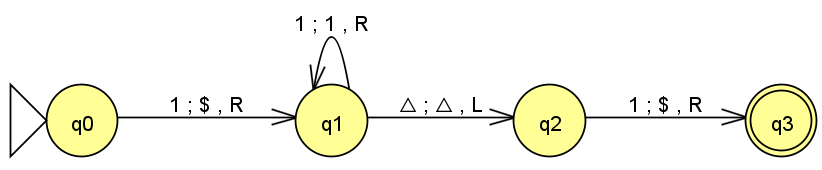
\includegraphics[width=0.7\paperwidth,keepaspectratio]{../../../images/turing/fx_x-2.png}%
\end{center}

\textbf{مثال على حالات الشريط ($x = 5$):}

{\small
\textbf{المدخل:}
\hfill
    \begin{tikzpicture}[scale=0.85]
        \foreach \i/\c in {1/$\vdash$,2/1,3/1,4/1,5/1,6/1,7/$\triangle$} {
            \draw (\i,0) rectangle +(1,0.8);
            \node at (\i+0.5,0.4) {\c};
            }
            \node at (8.5, 0.4) {$\ldots$};
    \end{tikzpicture}

\textbf{$q_0$: تحوّل أول $1$ إلى $\$$، تنتقل لـ $q_1$:}
\hfill
\begin{tikzpicture}[scale=0.85]
    \foreach \i/\c in {1/$\vdash$,2/$\$$,3/1,4/1,5/1,6/1,7/$\triangle$} {
        \draw (\i,0) rectangle +(1,0.8);
        \node at (\i+0.5,0.4) {\c};
    }
    \draw[->, thick, red] (3.5,1.5) -- (3.5,0.8);
    \node[red, font=\small] at (3.5,1.9) {$q_1$};
\end{tikzpicture}

\vspace{0.6em}
\textbf{$q_1$: يتجاوز الـ $1$ حتى $\triangle$، يرجع $q_2$:}
\hfill
\begin{tikzpicture}[scale=0.85]
    \foreach \i/\c in {1/$\vdash$,2/$\$$,3/1,4/1,5/1,6/1,7/$\triangle$} {
        \draw (\i,0) rectangle +(1,0.8);
        \node at (\i+0.5,0.4) {\c};
    }
    \draw[->, thick, blue] (6.5,1.5) -- (6.5,0.8);
\end{tikzpicture}

\vspace{0.6em}
\textbf{$q_2$: تحوّل آخر $1$ إلى $\$$، نهاية الناتج:}
\hfill
\begin{tikzpicture}[scale=0.85]
    \foreach \i/\c in {1/$\vdash$,2/$\$$,3/1,4/1,5/1,6/$\$$,7/$\triangle$} {
        \draw (\i,0) rectangle +(1,0.8);
        \node at (\i+0.5,0.4) {\c};
    }
    \node at (8.5, 0.4) {$\ldots$};
\end{tikzpicture}
} \\

$\leftarrow$ الناتج بين الـ\$: $1\,1\,1 (= 3 = 5-2)$ \checkmark \\

\textbf{شرح الحالات:}
\begin{itemize}
    \item $q_0$: حوّل أول $1$ إلى $\$$ (بداية الناتج) وانتقل لـ $q_1$.
    \item $q_1$: تجاوز باقي الـ $1$ يمينًا. عند $\triangle$: ارجع خطوة يسارًا ($q_2$).
    \item $q_2$: حوّل آخر $1$ إلى $\$$ (نهاية الناتج) واقبل.
    \item $q_3$: حالة القبول.
\end{itemize}

\begin{boxNote}
الآلة تعمل لـ $x \geq 2$ فقط. عند $x = 2$ يكون الناتج $\$\,\$$ (صفر وحدات بين الـ\$). عند $x < 2$ لا تتوقف الآلة بشكل صحيح لأنها غير مُعرَّفة لهذه الحالات.
\end{boxNote}

\textbf{تتبع ($x = 4$):}
\begin{align*}
q_0 \quad &\vdash \; \underline{1} \; 1 \; 1 \; 1 \; \triangle \\
q_1 \quad &\vdash \; \$ \; \underline{1} \; 1 \; 1 \; \triangle \quad \text{(حوّلنا $1$ الأولى إلى $\$$)} \\
q_1 \quad &\vdash \; \$ \; 1 \; \underline{1} \; 1 \; \triangle \\
q_1 \quad &\vdash \; \$ \; 1 \; 1 \; \underline{1} \; \triangle \\
q_1 \quad &\vdash \; \$ \; 1 \; 1 \; 1 \; \underline{\triangle} \quad \text{(رأينا $\triangle$، رجعنا)} \\
q_2 \quad &\vdash \; \$ \; 1 \; 1 \; \underline{1} \; \triangle \\
q_3 \quad &\vdash \; \$ \; 1 \; 1 \; \$ \; \triangle \quad \checkmark \quad \text{(حوّلنا آخر $1$ إلى $\$$)}
\end{align*}

الناتج بين الـ\$: $1\,1$ (= 2 = 4-2) \checkmark

\textbf{تتبع ($x = 2$):}
\begin{align*}
q_0 \quad &\vdash \; \underline{1} \; 1 \; \triangle \\
q_1 \quad &\vdash \; \$ \; \underline{1} \; \triangle \\
q_1 \quad &\vdash \; \$ \; 1 \; \underline{\triangle} \quad \text{(رجعنا)} \\
q_2 \quad &\vdash \; \$ \; \underline{1} \; \triangle \\
q_3 \quad &\vdash \; \$ \; \$ \; \triangle \quad \checkmark \quad \text{(ناتج = 0)}
\end{align*}

\clearpage

\subsection{مثال 8: حساب دالة $f(x) = x + 1$}

\textbf{المطلوب:} بناء آلة تيورينج تحسب الدالة $f(x) = x + 1$ لـ $x \geq 0$.

\medskip
\textbf{الفكرة:}

نحوّل أول $1$ إلى $\$$ (بداية الناتج)، ثم نتجاوز باقي الـ $1$ يمينًا، ونضيف وحدتين ($1\,1$) في نهاية الشريط، ثم نكتب $\$$. الوحدات بين الـ$\$$ = $(x-1) + 2 = x+1$.

\begin{center}
    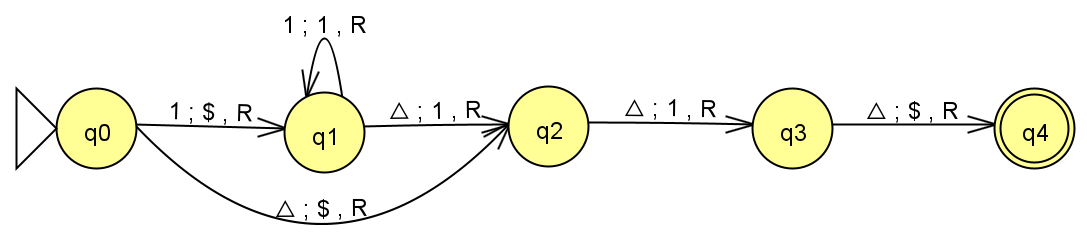
\includegraphics[width=0.7\paperwidth,keepaspectratio]{../../../images/turing/fx_xPlus1.png}%
\end{center}

\textbf{مثال على حالات الشريط ($x = 3$):} \\

{ \small
\textbf{المدخل:}
\hfill
\begin{tikzpicture}[scale=0.85]
    \foreach \i/\c in {1/$\vdash$,2/1,3/1,4/1,5/$\triangle$} {
        \draw (\i,0) rectangle +(1,0.8);
        \node at (\i+0.5,0.4) {\c};
    }
    \node at (6.5, 0.4) {$\ldots$};
\end{tikzpicture}

\textbf{$q_0 \to q_1$: أول $1$ تصبح $\$$:}
\hfill
\begin{tikzpicture}[scale=0.85]
    \foreach \i/\c in {1/$\vdash$,2/$\$$,3/1,4/1,5/$\triangle$} {
        \draw (\i,0) rectangle +(1,0.8);
        \node at (\i+0.5,0.4) {\c};
    }
    \draw[->, thick, red] (3.5,1.5) -- (3.5,0.8);
    \node[red, font=\small] at (3.5,1.9) {$q_1$};
\end{tikzpicture}

\textbf{$q_1 \to q_2 \to q_3$: تجاوز الـ$1$، إضافة $1\,1$:}
\hfill
\begin{tikzpicture}[scale=0.85]
    \foreach \i/\c in {1/$\vdash$,2/$\$$,3/1,4/1,5/1,6/1,7/$\triangle$} {
        \draw (\i,0) rectangle +(1,0.8);
        \node at (\i+0.5,0.4) {\c};
    }
    \draw[->, thick, blue] (7.5,1.5) -- (7.5,0.8);
    \node[blue, font=\small] at (7.5,1.9) {$q_3$};
\end{tikzpicture}

\vspace{0.6em}
\textbf{$q_3 \to q_4$: كتابة $\$$ النهاية:}
\hfill
\begin{tikzpicture}[scale=0.85]
    \foreach \i/\c in {1/$\vdash$,2/$\$$,3/1,4/1,5/1,6/1,7/$\$$} {
        \draw (\i,0) rectangle +(1,0.8);
        \node at (\i+0.5,0.4) {\c};
    }
    \node at (8.5, 0.4) {$\ldots$};
\end{tikzpicture}
} \\

$\leftarrow$ الناتج بين الـ\$: $1\,1\,1\,1$ (= 4 = 3+1) \checkmark \\

\textbf{شرح الحالات:}
\begin{itemize}
    \item $q_0$: حوّل أول $1$ إلى $\$$ (بداية الناتج) وانتقل لـ $q_1$. إذا كان الشريط فارغًا (أي $x=0$)، عندها اكتب $\$$ وانتقل للحالة $q2$ (التي ستضيف $1$ ثم $\$$ ثم تقبل)
    \item $q_1$: تجاوز باقي الـ $1$ يمينًا. عند $\triangle$: اكتب $1$ إضافية (أولى) وانتقل لـ $q_2$.
    \item $q_2$: اكتب $1$ إضافية (ثانية) وانتقل لـ $q_3$.
    \item $q_3$: اكتب $\$$ (نهاية الناتج) واقبل.
    \item $q_4$: حالة القبول.
\end{itemize}

\begin{boxNote}
الناتج = $(x-1)$ وحدة أصلية $+$ وحدتان مضافتان $x+1 =$. الآلة تعمل لـ $x \geq 0$.
\end{boxNote}

\textbf{تتبع ($x = 3$):}
\begin{align*}
q_0 \quad &\vdash \; \underline{1} \; 1 \; 1 \; \triangle \\
q_1 \quad &\vdash \; \$ \; \underline{1} \; 1 \; \triangle \quad \text{(أول $1$ أصبحت $\$$)} \\
q_1 \quad &\vdash \; \$ \; 1 \; \underline{1} \; \triangle \\
q_1 \quad &\vdash \; \$ \; 1 \; 1 \; \underline{\triangle} \\
q_2 \quad &\vdash \; \$ \; 1 \; 1 \; 1 \; \underline{\triangle} \quad \text{(أضفنا $1$ أولى)} \\
q_3 \quad &\vdash \; \$ \; 1 \; 1 \; 1 \; 1 \; \underline{\triangle} \quad \text{(أضفنا $1$ ثانية)} \\
q_4 \quad &\vdash \; \$ \; 1 \; 1 \; 1 \; 1 \; \$ \quad \checkmark \quad \text{(الناتج $4 = 3+1$)}
\end{align*}

الناتج بين الـ\$: $1\,1\,1\,1$ (= 4 = 3+1) \checkmark

\clearpage

\subsection{مثال 9: حساب دالة $f(x) = 2x$}

\textbf{المطلوب:} بناء آلة تيورينج تحسب الدالة $f(x) = 2x$.

\medskip
\textbf{الفكرة:}

\begin{enumerate}
    \item ضع علامة $\$$ في نهاية المدخل (فاصل بين المدخل ومنطقة الناتج)، وارجع لبداية الشريط.
    \item في كل دورة: حوّل أول $1$ غير مُعالَجة إلى $X$، ثم اذهب لنهاية الناتج وأضف $1\,1$.
    \item عندما لا تبقى $1$ في المدخل (وصلت إلى $\$$): اذهب لنهاية الناتج واكتب $\$$ (نهاية الناتج).
\end{enumerate}

الناتج النهائي: بين \$ الأولى و\$ الثانية.

\begin{center}
    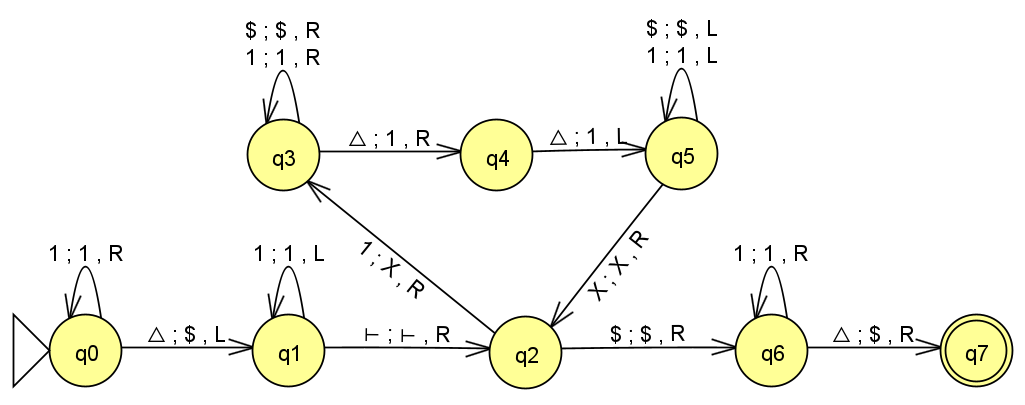
\includegraphics[width=0.7\paperwidth,keepaspectratio]{../../../images/turing/fx_2x.png}%
\end{center}

\textbf{مثال على حالات الشريط ($x = 2$):} \\

{ \small

\textbf{المدخل:}
\hfill
\begin{tikzpicture}[scale=0.83]
    \foreach \i/\c in {1/$\vdash$,2/1,3/1,4/$\triangle$} {
        \draw (\i,0) rectangle +(1,0.8);
        \node at (\i+0.5,0.4) {\c};
    }
    \node at (5.5, 0.4) {$\ldots$};
\end{tikzpicture}

\textbf{$q_0$: تجاوز المدخل، كتابة $\$$ في النهاية، رجوع ($q_1 \to q_2$):}
\hfill
\begin{tikzpicture}[scale=0.83]
    \foreach \i/\c in {1/$\vdash$,2/1,3/1,4/$\$$,5/$\triangle$} {
        \draw (\i,0) rectangle +(1,0.8);
        \node at (\i+0.5,0.4) {\c};
    }
\end{tikzpicture}

\textbf{دورة 1: $1 \to X$، إضافة $1\,1$ بعد $\$$:}
\hfill
\begin{tikzpicture}[scale=0.83]
    \foreach \i/\c in {1/$\vdash$,2/$X$,3/1,4/$\$$,5/1,6/1,7/$\triangle$} {
        \draw (\i,0) rectangle +(1,0.8);
        \node at (\i+0.5,0.4) {\c};
    }
\end{tikzpicture}

\textbf{دورة 2: $1 \to X$، إضافة $1\,1$ بعد $\$$:}
\hfill
\begin{tikzpicture}[scale=0.83]
    \foreach \i/\c in {1/$\vdash$,2/$X$,3/$X$,4/$\$$,5/1,6/1,7/1,8/1,9/$\triangle$} {
        \draw (\i,0) rectangle +(1,0.8);
        \node at (\i+0.5,0.4) {\c};
    }
\end{tikzpicture}

\textbf{الناتج النهائي ($q_2$ يرى $\$$، يكتب $\$$ في النهاية):}
\hfill
\begin{tikzpicture}[scale=0.83]
    \foreach \i/\c in {1/$\vdash$,2/$X$,3/$X$,4/$\$$,5/1,6/1,7/1,8/1,9/$\$$} {
        \draw (\i,0) rectangle +(1,0.8);
        \node at (\i+0.5,0.4) {\c};
    }
    \node at (10.5, 0.4) {$\ldots$};
\end{tikzpicture}
} \\

$\leftarrow$ الناتج بين الـ\$: $1\,1\,1\,1$ (= 4 = 2 \texttimes 2) \checkmark \\
\clearpage
\textbf{شرح الحالات:}
\begin{itemize}
    \item $q_0$: تجاوز المدخل يمينًا. عند $\triangle$: اكتب $\$$ (فاصل الناتج) وارجع يسارًا ($q_1$).
    \item $q_1$: ارجع يسارًا حتى $\vdash$، ثم تقدم لـ $q_2$ (بداية دورة جديدة).
    \item $q_2$: إذا $1$: حوّلها $X$ وانتقل لـ $q_3$ (كتابة $11$ في الناتج). إذا $\$$: انتهى المدخل، اذهب لـ $q_6$.
    \item $q_3$: تجاوز $1$s و$\$$s يمينًا حتى $\triangle$، اكتب $1$ الأولى ($q_4$).
    \item $q_4$: اكتب $1$ الثانية وارجع يسارًا ($q_5$).
    \item $q_5$: ارجع يسارًا على $1$s و$\$$s حتى $X$، ثم تقدم لدورة جديدة ($q_2$).
    \item $q_6$: تجاوز الناتج يمينًا حتى $\triangle$، اكتب $\$$ (نهاية الناتج) واقبل ($q_7$).
\end{itemize}

\textbf{تتبع ($x = 2$):}
{\small
\begin{align*}
q_0 \quad &\vdash \; \underline{1} \; 1 \; \triangle \\
q_0 \quad &\vdash \; 1 \; \underline{1} \; \triangle \\
q_0 \quad &\vdash \; 1 \; 1 \; \underline{\triangle} \quad \text{(كتبنا $\$$، رجعنا)} \\
q_1 \quad &\vdash \; 1 \; \underline{1} \; \$ \; \triangle \\
q_1 \quad &\vdash \; \underline{1} \; 1 \; \$ \; \triangle \\
q_1 \quad &\vdash \; \underline{\vdash} \; 1 \; 1 \; \$ \; \triangle \\
q_2 \quad &\vdash \; \underline{1} \; 1 \; \$ \; \triangle \quad \text{($1 \to X$)} \\
q_3 \quad &\vdash \; X \; \underline{1} \; \$ \; \triangle \quad \text{(تجاوز $1$, $\$$)} \\
q_3 \quad &\vdash \; X \; 1 \; \underline{\$} \; \triangle \\
q_3 \quad &\vdash \; X \; 1 \; \$ \; \underline{\triangle} \quad \text{(كتبنا $1$ أولى)} \\
q_4 \quad &\vdash \; X \; 1 \; \$ \; 1 \; \underline{\triangle} \quad \text{(كتبنا $1$ ثانية، رجعنا)} \\
q_5 \quad &\vdash \; X \; 1 \; \$ \; \underline{1} \; 1 \\
q_5 \quad &\vdash \; X \; 1 \; \underline{\$} \; 1 \; 1 \\
q_5 \quad &\vdash \; X \; \underline{1} \; \$ \; 1 \; 1 \\
q_5 \quad &\vdash \; \underline{X} \; 1 \; \$ \; 1 \; 1 \quad \text{(وجدنا $X$، تقدمنا)} \\
q_2 \quad &\vdash \; X \; \underline{1} \; \$ \; 1 \; 1 \quad \text{($1 \to X$)} \\
q_3 \quad &\vdash \; X \; X \; \underline{\$} \; 1 \; 1 \; \triangle \\
q_3 \quad &\vdash \; X \; X \; \$ \; \underline{1} \; 1 \; \triangle \\
q_3 \quad &\vdash \; X \; X \; \$ \; 1 \; \underline{1} \; \triangle \\
q_3 \quad &\vdash \; X \; X \; \$ \; 1 \; 1 \; \underline{\triangle} \quad \text{(كتبنا $1$ ثالثة)} \\
q_4 \quad &\vdash \; X \; X \; \$ \; 1 \; 1 \; 1 \; \underline{\triangle} \quad \text{(كتبنا $1$ رابعة، رجعنا)} \\
q_5 \quad &\vdash \; X \; \underline{X} \; \$ \; 1 \; 1 \; 1 \; 1 \quad \text{(وجدنا $X$، تقدمنا)} \\
q_2 \quad &\vdash \; X \; X \; \underline{\$} \; 1 \; 1 \; 1 \; 1 \quad \text{($q_2$ يرى $\$$: المدخل انتهى)} \\
q_6 \quad &\vdash \; X \; X \; \$ \; \underline{1} \; 1 \; 1 \; 1 \; \triangle \\
q_6 \quad &\vdash \; X \; X \; \$ \; 1 \; 1 \; 1 \; 1 \; \underline{\triangle} \quad \text{(كتبنا $\$$ النهائية)} \\
q_7 \quad &\vdash \; X \; X \; \$ \; 1 \; 1 \; 1 \; 1 \; \$ \quad \checkmark
\end{align*}
}
الناتج بين الـ\$: $1\,1\,1\,1$ (= 4 = 2 \texttimes 2) \checkmark

\clearpage

%=============================================================
\subsection{مثال 10: حساب دالة $f(x) = x/3$}
%=============================================================

\textbf{المطلوب:} بناء آلة تيورينج تحسب الدالة $f(x) = x/3$.

\textbf{الفكرة:}

نفس أسلوب مثال $2x$، لكن معكوسًا: بدلاً من كتابة $1\,1$ لكل $1$ مُعالَجة، نشطب $3$ وحدات لكتابة $1$ واحدة في الناتج.

\begin{enumerate}
    \item ضع $\$$ في نهاية المدخل (فاصل)، وارجع لبداية الشريط.
    \item في كل دورة: حوّل ثلاث $1$ متتالية إلى $X\,X\,X$، ثم اذهب لنهاية الناتج وأضف $1$.
    \item عندما لا تبقى $1$ في المدخل (وصلت $\$$): اكتب $\$$ نهاية الناتج واقبل.
\end{enumerate}


\begin{center}
    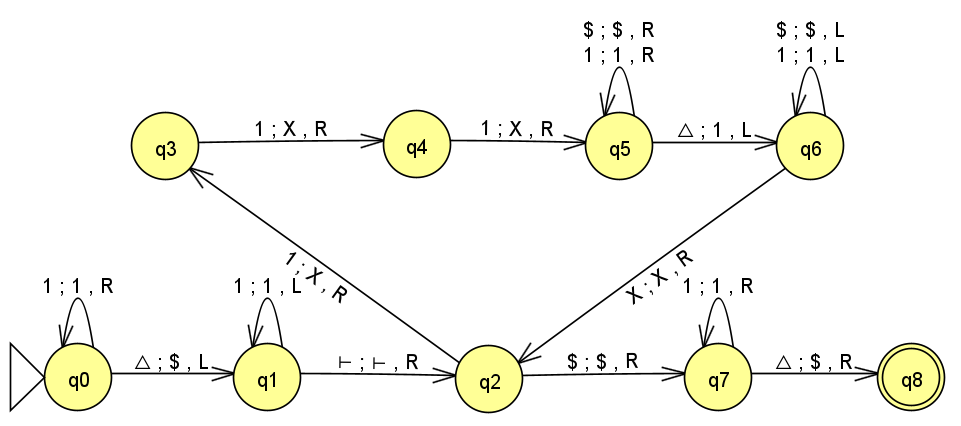
\includegraphics[width=0.7\paperwidth,keepaspectratio]{../../../images/turing/fx_xDiv3.png}%
\end{center}

\textbf{مثال على حالات الشريط ($x = 6$):} \\

{\small
\textbf{المدخل:}
\hfill
\begin{tikzpicture}[scale=0.83]
    \foreach \i/\c in {1/$\vdash$,2/1,3/1,4/1,5/1,6/1,7/1,8/$\triangle$} {
        \draw (\i,0) rectangle +(1,0.8);
        \node at (\i+0.5,0.4) {\c};
    }
\end{tikzpicture}

\textbf{بعد الإعداد: $\$$ في النهاية:}
\hfill
\begin{tikzpicture}[scale=0.83]
    \foreach \i/\c in {1/$\vdash$,2/1,3/1,4/1,5/1,6/1,7/1,8/$\$$,9/$\triangle$} {
        \draw (\i,0) rectangle +(1,0.8);
        \node at (\i+0.5,0.4) {\c};
    }
\end{tikzpicture}

\textbf{دورة 1: شطب $3$، كتابة $1$ في الناتج:}
\hfill
\begin{tikzpicture}[scale=0.83]
    \foreach \i/\c in {1/$\vdash$,2/$X$,3/$X$,4/$X$,5/1,6/1,7/1,8/$\$$,9/1,10/$\triangle$} {
        \draw (\i,0) rectangle +(1,0.8);
        \node at (\i+0.5,0.4) {\c};
    }
\end{tikzpicture}

\textbf{الناتج النهائي:}
\hfill
\begin{tikzpicture}[scale=0.83]
    \foreach \i/\c in {1/$\vdash$,2/$X$,3/$X$,4/$X$,5/$X$,6/$X$,7/$X$,8/$\$$,9/1,10/1,11/$\$$} {
        \draw (\i,0) rectangle +(1,0.8);
        \node at (\i+0.5,0.4) {\c};
    }
    \node at (12.5, 0.4) {$\ldots$};
\end{tikzpicture}
} \\

$\leftarrow$ الناتج بين الـ\$: $1\,1$ (= 2 = 6/3) \checkmark \\

\clearpage
\textbf{شرح الحالات:}
\begin{itemize}
    \item $q_0$: تجاوز المدخل يمينًا. عند $\triangle$: اكتب $\$$ وارجع ($q_1$).
    \item $q_1$: ارجع حتى $\vdash$، تقدم لـ $q_2$.
    \item $q_2$: إذا $1$: ابدأ شطب ثلاث ($q_3$). إذا $\$$: المدخل انتهى ← $q_7$.
    \item $q_3, q_4$: شطب الثانية والثالثة (كل منهما $1 \mid X, R$).
    \item $q_5$: تجاوز الناتج حتى $\triangle$، اكتب $1$ واحدة في الناتج وارجع ($q_6$).
    \item $q_6$: ارجع لبداية الشريط وابدأ دورة جديدة.
    \item $q_7$: تجاوز الناتج حتى $\triangle$، اكتب $\$$ (نهاية الناتج) واقبل ($q_8$).
\end{itemize}

\textbf{تتبع ($x = 3$):}
{ \small
\begin{align*}
q_0 \quad &\vdash \; \underline{1} \; 1 \; 1 \; \triangle \\
q_0 \quad &\vdash \; 1 \; 1 \; 1 \; \underline{\triangle} \quad \text{(كتبنا $\$$، رجعنا)} \\
q_1 \quad &\vdash \; \underline{\vdash} \; 1 \; 1 \; 1 \; \$ \; \triangle \\
q_2 \quad &\vdash \; \underline{1} \; 1 \; 1 \; \$ \; \triangle \quad \text{($1 \to X$)} \\
q_3 \quad &\vdash \; X \; \underline{1} \; 1 \; \$ \; \triangle \quad \text{($1 \to X$)} \\
q_4 \quad &\vdash \; X \; X \; \underline{1} \; \$ \; \triangle \quad \text{($1 \to X$)} \\
q_5 \quad &\vdash \; X \; X \; X \; \underline{\$} \; \triangle \quad \text{(تجاوز $\$$)} \\
q_5 \quad &\vdash \; X \; X \; X \; \$ \; \underline{\triangle} \quad \text{(كتبنا $1$، رجعنا)} \\
q_b \quad &\vdash \; \underline{\vdash} \; X \; X \; X \; \$ \; 1 \\
q_2 \quad &\vdash \; X \; \underline{X} \; X \; \$ \; 1 \quad \text{... (يتجاوز Xs)} \\
q_2 \quad &\vdash \; X \; X \; X \; \underline{\$} \; 1 \quad \text{($q_2$ يرى $\$$: انتهى)} \\
q_6 \quad &\vdash \; X \; X \; X \; \$ \; \underline{1} \; \triangle \\
q_6 \quad &\vdash \; X \; X \; X \; \$ \; 1 \; \underline{\triangle} \quad \text{(كتبنا $\$$)} \\
q_7 \quad &\vdash \; X \; X \; X \; \$ \; 1 \; \$ \quad \checkmark
\end{align*}
}

الناتج بين الـ\$: $1$ (= 1 = 3/3) \checkmark

\clearpage

\subsection{مثال 11: حساب دالة $f(x) = x \% 3$}
%=============================================================

\textbf{المطلوب:} بناء آلة تيورينج تحسب الدالة $f(x) = x \% 3$ للأعداد الطبيعية $x \geq 0$.

\textbf{الناتج:} العدد $x \% 3 \in \{0, 1, 2\}$ بالتمثيل الأوناري، محاطًا بـ $\$$.

\begin{center}
    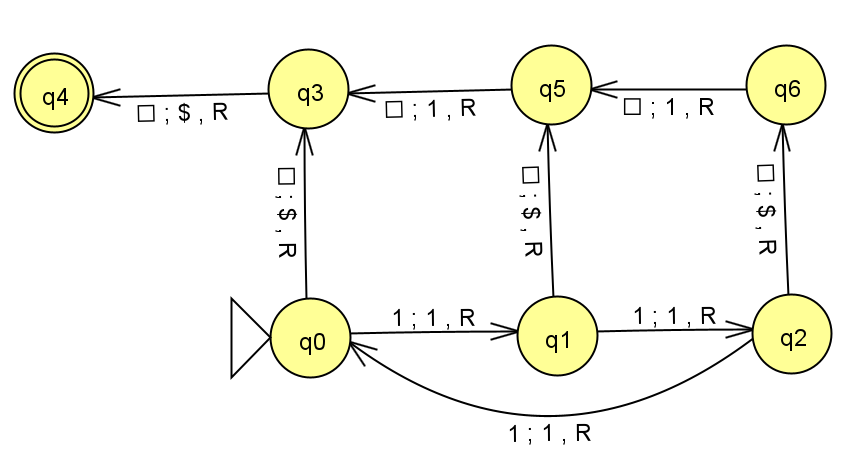
\includegraphics[width=0.6\paperwidth,keepaspectratio]{../../../images/turing/fx_xMod3.png}%
\end{center}

\textbf{الفكرة (مرور واحد + تشفير الباقي في الحالة):}

تمر الآلة على المدخل \textbf{مرة واحدة فقط} يمينًا. الحالات $q_0, q_1, q_2$ تتناوب دوريًا مع كل $1$ مقروءة، وكل حالة تمثل الباقي الجزئي الحالي:

\begin{center}
\begin{tabular}{c|c}
الحالة & الباقي الحالي لعدد الـ $1$ المقروءة \\
\hline
$q_0$ & $0$ \\
$q_1$ & $1$ \\
$q_2$ & $2$ \\
\end{tabular}
\end{center}

عند الوصول لـ $\triangle$، تعرف الآلة الباقي النهائي من الحالة الحالية، فتكتب الناتج مباشرةً بعد المدخل:

\begin{center}
\begin{tabular}{c|c|c}
الحالة عند $\triangle$ & الباقي & الناتج المكتوب على الشريط \\
\hline
$q_0$ & $0$ & $\$\,\$$ \\
$q_1$ & $1$ & $\$\,1\,\$$ \\
$q_2$ & $2$ & $\$\,1\,1\,\$$ \\
\end{tabular}
\end{center}

\textbf{مثال على حالات الشريط ($x = 4$، الباقي $= 1$):} \\

{\small
\textbf{المدخل:}
\hfill
\begin{tikzpicture}[scale=0.83]
    \foreach \i/\c in {1/$\vdash$,2/1,3/1,4/1,5/1,6/$\triangle$} {
        \draw (\i,0) rectangle +(1,0.8);
        \node at (\i+0.5,0.4) {\c};
    }
\end{tikzpicture}

\textbf{بعد قراءة المدخل (حالة $q_1$، باقي $= 1$):}
\hfill
\begin{tikzpicture}[scale=0.83]
    \foreach \i/\c in {1/$\vdash$,2/1,3/1,4/1,5/1,6/$\triangle$} {
        \draw (\i,0) rectangle +(1,0.8);
        \node at (\i+0.5,0.4) {\c};
    }
    \draw[->, thick, red] (6.5,1.5) -- (6.5,0.8);
    \node[red, font=\small] at (6.5,1.9) {$q_1$, باقي $= 1$};
\end{tikzpicture}

\textbf{الناتج النهائي:}
\hfill
\begin{tikzpicture}[scale=0.83]
    \foreach \i/\c in {1/$\vdash$,2/1,3/1,4/1,5/1,6/$\$$,7/1,8/$\$$} {
        \draw (\i,0) rectangle +(1,0.8);
        \node at (\i+0.5,0.4) {\c};
    }
    \node at (9.5, 0.4) {$\ldots$};
\end{tikzpicture}
} \\

$\leftarrow$ الناتج بين الـ\$: $1$ (= 1 = 4 \% 3) \checkmark \\

\medskip
\textbf{شرح الحالات:}
\begin{itemize}
    \item $q_0$: الباقي الحالي $= 0$. قراءة $1$: انتقل لـ $q_1$. قراءة $\triangle$: اكتب $\$$ وانتقل لـ $q_3$ (ناتج فارغ).
    \item $q_1$: الباقي الحالي $= 1$. قراءة $1$: انتقل لـ $q_2$. قراءة $\triangle$: اكتب $\$$ وانتقل لـ $q_5$.
    \item $q_2$: الباقي الحالي $= 2$. قراءة $1$: انتقل لـ $q_0$ (دورة كاملة). قراءة $\triangle$: اكتب $\$$ وانتقل لـ $q_6$.
    \item $q_3$: اكتب $\$$ الإغلاق واقبل ($q_4$).
    \item $q_5$: اكتب $1$ واحدة ثم انتقل لـ $q_3$.
    \item $q_6$: اكتب $1$ الأولى ثم انتقل لـ $q_5$.
    \item $q_4$: حالة القبول.
\end{itemize}

\begin{boxNote}
\textbf{جمال هذه الآلة:} مرور واحد فقط على المدخل، بدون شطب أو رجوع. الحالات $q_0, q_1, q_2$ تعمل كـ``ذاكرة'' تحفظ الباقي الجزئي أولاً بأول. هذه التقنية تُسمى \textbf{تشفير المعلومات في الحالة} وهي واحدة من أقوى أدوات تصميم آلات تيورينج.
\end{boxNote}

\textbf{تتبع ($x = 5$، $5 \% 3 = 2$):}
\begin{align*}
q_0 \quad &\vdash \; \underline{1} \; 1 \; 1 \; 1 \; 1 \; \triangle \\
q_1 \quad &\vdash \; 1 \; \underline{1} \; 1 \; 1 \; 1 \; \triangle \\
q_2 \quad &\vdash \; 1 \; 1 \; \underline{1} \; 1 \; 1 \; \triangle \\
q_0 \quad &\vdash \; 1 \; 1 \; 1 \; \underline{1} \; 1 \; \triangle \\
q_1 \quad &\vdash \; 1 \; 1 \; 1 \; 1 \; \underline{1} \; \triangle \\
q_2 \quad &\vdash \; 1 \; 1 \; 1 \; 1 \; 1 \; \underline{\triangle} \quad \text{(باقي $= 2$، اكتب $\$$)} \\
q_6 \quad &\vdash \; 1 \; 1 \; 1 \; 1 \; 1 \; \$ \; \underline{\triangle} \quad \text{(اكتب $1$ أولى → $q_5$)} \\
q_5 \quad &\vdash \; 1 \; 1 \; 1 \; 1 \; 1 \; \$ \; 1 \; \underline{\triangle} \quad \text{(اكتب $1$ ثانية → $q_3$)} \\
q_3 \quad &\vdash \; 1 \; 1 \; 1 \; 1 \; 1 \; \$ \; 1 \; 1 \; \underline{\triangle} \\
q_4 \quad &\vdash \; 1 \; 1 \; 1 \; 1 \; 1 \; \$ \; 1 \; 1 \; \$ \quad \checkmark
\end{align*}

الناتج بين الـ\$: $1\,1$ (= 2 = 5 \% 3) \checkmark

\textbf{تتبع ($x = 3$، $3 \% 3 = 0$):}
\begin{align*}
q_0 \to q_1 \to q_2 \to q_0 \quad &\vdash \; 1 \; 1 \; 1 \; \underline{\triangle} \quad \text{(باقي $= 0$، اكتب $\$$)} \\
q_3 \quad &\vdash \; 1 \; 1 \; 1 \; \$ \; \underline{\triangle} \quad \text{(اكتب $\$$ الإغلاق)} \\
q_4 \quad &\vdash \; 1 \; 1 \; 1 \; \$ \; \$ \quad \checkmark \quad \text{(ناتج $= 0$)}
\end{align*}

\clearpage

%=============================================================

\subsection{مثال 12: حساب دالة $f(x,y) = x + y$}
%=============================================================

\textbf{المطلوب:} بناء آلة تيورينج تحسب $f(x, y) = x + y$.

\textbf{المدخل:} $\vdash \underbrace{1\ldots1}_{x} \# \underbrace{1\ldots1}_{y} \triangle$

\textbf{الناتج:} العدد $x+y$ بالتمثيل الأوناري بين $\$$ و $\$$.

\begin{center}
    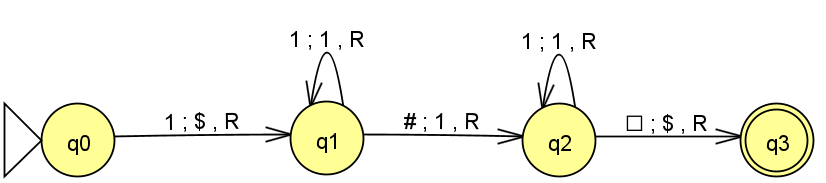
\includegraphics[width=0.7\paperwidth,keepaspectratio]{../../../images/turing/fx_XplusY.png}%
\end{center}

\textbf{الفكرة (مرور واحد من اليسار لليمين):}

الآلة تمر على الشريط مرة واحدة فقط يمينًا دون رجوع:
\begin{enumerate}
    \item أول $1$ في $x$ تصبح $\$$ (بداية الناتج) وتنتقل لـ $q_1$.
    \item باقي $1$s في $x$ تُترك كما هي ($q_1$ يتجاوزها).
    \item الفاصل $\#$ يصبح $1$ (لتعويض الوحدة التي حوّلناها $\$$ في الخطوة 1)، وتنتقل لـ $q_2$.
    \item $1$s في $y$ تُترك كما هي ($q_2$ يتجاوزها).
    \item عند $\triangle$: تُكتب $\$$ (نهاية الناتج) ويُقبل.
\end{enumerate}

النتيجة: بين الـ$\$$s يوجد $(x-1)$ وحدة من $x$ + وحدة واحدة من تحويل $\#$ + $y$ وحدة $= x + y$ \checkmark

\textbf{مثال على حالات الشريط ($x=2, y=3$):} \\

{\small
\textbf{المدخل:}
\hfill
\begin{tikzpicture}[scale=0.83]
    \foreach \i/\c in {1/$\vdash$,2/1,3/1,4/$\#$,5/1,6/1,7/1,8/$\triangle$} {
        \draw (\i,0) rectangle +(1,0.8);
        \node at (\i+0.5,0.4) {\c};
    }
\end{tikzpicture}

\textbf{$q_0$: أول $1$ تصبح $\$$، انتقال لـ $q_1$:}
\hfill
\begin{tikzpicture}[scale=0.83]
    \foreach \i/\c in {1/$\vdash$,2/$\$$,3/1,4/$\#$,5/1,6/1,7/1,8/$\triangle$} {
        \draw (\i,0) rectangle +(1,0.8);
        \node at (\i+0.5,0.4) {\c};
    }
    \draw[->, thick, red] (3.5,1.5) -- (3.5,0.8);
    \node[red, font=\small] at (3.5,1.9) {$q_1$};
\end{tikzpicture}

\textbf{$q_1$: تجاوز $1$، وصل $\#$ ← $\#$ يصبح $1$، انتقال لـ $q_2$:}
\hfill
\begin{tikzpicture}[scale=0.83]
    \foreach \i/\c in {1/$\vdash$,2/$\$$,3/1,4/1,5/1,6/1,7/1,8/$\triangle$} {
        \draw (\i,0) rectangle +(1,0.8);
        \node at (\i+0.5,0.4) {\c};
    }
    \draw[->, thick, blue] (5.5,1.5) -- (5.5,0.8);
    \node[blue, font=\small] at (5.5,1.9) {$q_2$};
\end{tikzpicture}

\textbf{$q_2$: تجاوز $1,1,1$، وصل $\triangle$ ← كتابة $\$$، قبول:}
\hfill
\begin{tikzpicture}[scale=0.83]
    \foreach \i/\c in {1/$\vdash$,2/$\$$,3/1,4/1,5/1,6/1,7/1,8/$\$$} {
        \draw (\i,0) rectangle +(1,0.8);
        \node at (\i+0.5,0.4) {\c};
    }
    \node at (9.5, 0.4) {$\ldots$};
\end{tikzpicture}
} \\

$\leftarrow$ الناتج بين الـ\$: $1\,1\,1\,1\,1$ (= 5 = 2+3) \checkmark \\

\medskip
\textbf{شرح الحالات:}
\begin{itemize}
    \item $q_0$: حوّل أول $1$ في $x$ إلى $\$$ (بداية الناتج) وانتقل لـ $q_1$.
    \item $q_1$: تجاوز باقي $1$s في $x$ يمينًا. عند $\#$: حوّله إلى $1$ (يعوّض الوحدة المفقودة) وانتقل لـ $q_2$.
    \item $q_2$: تجاوز $1$s في $y$ يمينًا. عند $\triangle$: اكتب $\$$ (نهاية الناتج) واقبل ($q_3$).
    \item $q_3$: حالة القبول.
\end{itemize}

\begin{boxNote}
\textbf{لماذا $\# \to 1$ يعطي الناتج الصحيح؟} الآلة تستهلك أول $1$ من $x$ لتصنع $\$$ البداية، فتفقد وحدة واحدة. تحويل $\#$ إلى $1$ يُعيد هذه الوحدة بالضبط. النتيجة: $(x-1) + 1 + y = x+y$. آلة من 4 حالات فقط، مرور واحد، بدون رجوع!
\end{boxNote}

\textbf{تتبع ($x=2, y=3$):}
\begin{align*}
q_0 \quad &\vdash \; \underline{1} \; 1 \; \# \; 1 \; 1 \; 1 \; \triangle
    \quad \text{($1 \to \$$)} \\
q_1 \quad &\vdash \; \$ \; \underline{1} \; \# \; 1 \; 1 \; 1 \; \triangle
    \quad \text{(تجاوز $1$)} \\
q_1 \quad &\vdash \; \$ \; 1 \; \underline{\#} \; 1 \; 1 \; 1 \; \triangle
    \quad \text{($\# \to 1$)} \\
q_2 \quad &\vdash \; \$ \; 1 \; 1 \; \underline{1} \; 1 \; 1 \; \triangle
    \quad \text{(تجاوز $1,1,1$)} \\
q_2 \quad &\vdash \; \$ \; 1 \; 1 \; 1 \; 1 \; 1 \; \underline{\triangle}
    \quad \text{(كتبنا $\$$)} \\
q_3 \quad &\vdash \; \$ \; 1 \; 1 \; 1 \; 1 \; 1 \; \$ \quad \checkmark
\end{align*}

الناتج بين الـ\$: $1\,1\,1\,1\,1$ (= 5 = 2+3) \checkmark

\textbf{تتبع ($x=1, y=2$):}
\begin{align*}
q_0 \quad &\vdash \; \underline{1} \; \# \; 1 \; 1 \; \triangle
    \quad \text{($1 \to \$$)} \\
q_1 \quad &\vdash \; \$ \; \underline{\#} \; 1 \; 1 \; \triangle
    \quad \text{($\# \to 1$، لا $1$s متبقية في $x$)} \\
q_2 \quad &\vdash \; \$ \; 1 \; \underline{1} \; 1 \; \triangle
    \quad \text{(تجاوز $1,1$)} \\
q_2 \quad &\vdash \; \$ \; 1 \; 1 \; 1 \; \underline{\triangle}
    \quad \text{(كتبنا $\$$)} \\
q_3 \quad &\vdash \; \$ \; 1 \; 1 \; 1 \; \$ \quad \checkmark
\end{align*}

الناتج بين الـ\$: $1\,1\,1$ (= 3 = 1+2) \checkmark

\clearpage


%%%%%%%%%%%%%%%%%%%%%%%%%%%%%%%%%%%%%%%%%%%%%%%%%%%%%%%%%%%%%%%%%%%%%%%%%%%%%%%%%%%%%%%%%%%%%%%%%%
\subsection{مثال 13: قبول اللغة $L = \{w \cdot R(w) \mid w \in \{a,b\}^*\}$}

\textbf{المطلوب:} بناء آلة تيورينج تقبل اللغة:
$$L = \{ w \cdot R(w) \mid w \in \{a, b\}^* \}$$

أي الكلمات المكوّنة بإلحاق كلمة $w$ بعكسها $R(w)$ مباشرةً (المتناظرات ذات الطول الزوجي).

\textbf{أمثلة:}
\begin{itemize}
    \item \textbf{مقبولة:} $\varepsilon,\; aa,\; bb,\; abba,\; baab,\; aabbaa$
    \item \textbf{مرفوضة:} $ab,\; aba,\; aabb,\; abab$
\end{itemize}

\begin{boxNote}
كل كلمة من الشكل $w \cdot R(w)$ هي متناظرة ذات طول زوجي. الحرف رقم $i$ من اليسار يساوي دائمًا الحرف رقم $i$ من اليمين.
\end{boxNote}

\begin{center}
    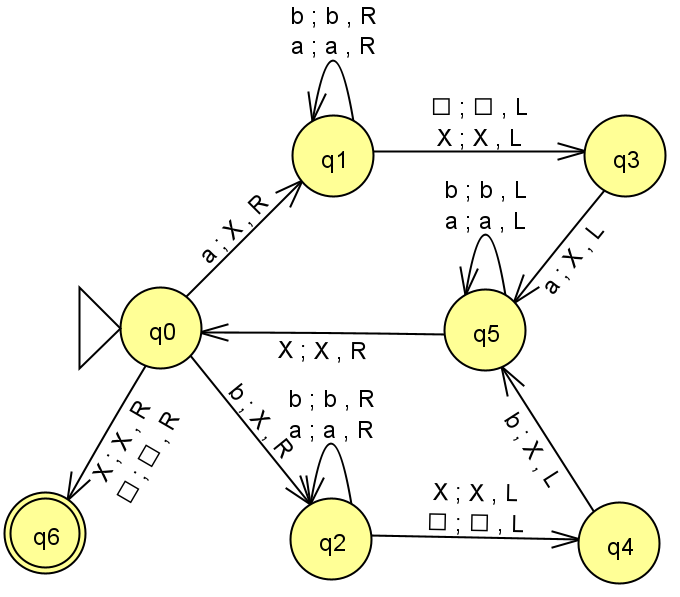
\includegraphics[width=0.5\paperwidth,keepaspectratio]{../../../images/turing/w_Rw_over_ab.png}%
\end{center}

\textbf{الفكرة (المقارنة من الطرفين):}

في كل دورة:
\begin{enumerate}
    \item اقرأ الحرف الأول غير مُعالَج وضع $X$ مكانه (الحالة تحفظ نوع الحرف: $q_1$ لـ $a$، $q_2$ لـ $b$).
    \item تجاوز بقية الأحرف غير المُعالَجة يمينًا حتى الطرف.
    \item تحرك خطوة يسارًا للوصول لآخر حرف غير مُعالَج، وتحقق أنه يطابق الحرف الأول:
        \begin{itemize}
            \item إذا تطابقا: ضع $X$ مكانه وارجع يسارًا ($q_5$).
            \item إذا اختلفا: لا انتقال → \textbf{رفض تلقائي}.
        \end{itemize}
    \item كرر حتى تُعالَج جميع الأحرف، ثم اقبل ($q_6$).
\end{enumerate}

\textbf{مثال على حالات الشريط ($w = ab$، المدخل $= abba$):} \\

{\small
\textbf{المدخل:}
\hfill
\begin{tikzpicture}[scale=0.85]
    \foreach \i/\c in {1/$\vdash$,2/a,3/b,4/b,5/a,6/$\triangle$} {
        \draw (\i,0) rectangle +(1,0.8);
        \node at (\i+0.5,0.4) {\c};
    }
\end{tikzpicture}

\textbf{دورة 1: $q_0$ يقرأ $a$، يضع $X$، يذهب يمينًا ($q_1$):}
\hfill
\begin{tikzpicture}[scale=0.85]
    \foreach \i/\c in {1/$\vdash$,2/$X$,3/b,4/b,5/a,6/$\triangle$} {
        \draw (\i,0) rectangle +(1,0.8);
        \node at (\i+0.5,0.4) {\c};
    }
    \draw[->, thick, red] (2.5,1.5) -- (2.5,0.8);
    \node[red, font=\small] at (2.5,1.9) {$q_1$ (تذكر $a$)};
\end{tikzpicture}

\textbf{$q_1$ تجاوز $b,b,a$ ← وصل $\triangle$، رجع يسارًا ($q_3$):}
\hfill
\begin{tikzpicture}[scale=0.85]
    \foreach \i/\c in {1/$\vdash$,2/$X$,3/b,4/b,5/a,6/$\triangle$} {
        \draw (\i,0) rectangle +(1,0.8);
        \node at (\i+0.5,0.4) {\c};
    }
    \draw[->, thick, blue] (5.5,1.5) -- (5.5,0.8);
    \node[blue, font=\small] at (5.5,1.9) {$q_3$ (يبحث $a$)};
\end{tikzpicture}

\textbf{$q_3$ وجد $a$ ← وضع $X$، رجع يسارًا ($q_5 \to q_0$):}
\hfill
\begin{tikzpicture}[scale=0.85]
    \foreach \i/\c in {1/$\vdash$,2/$X$,3/b,4/b,5/$X$,6/$\triangle$} {
        \draw (\i,0) rectangle +(1,0.8);
        \node at (\i+0.5,0.4) {\c};
    }
    \draw[->, thick, blue] (3.5,1.5) -- (3.5,0.8);
    \node[blue, font=\small] at (3.5,1.9) {$q_0$ يبدأ دورة 2};
\end{tikzpicture}

\textbf{دورة 2 مكتملة: $b$ من اليسار و $b$ من اليمين شُطبا:}
\hfill
\begin{tikzpicture}[scale=0.85]
    \foreach \i/\c in {1/$\vdash$,2/$X$,3/$X$,4/$X$,5/$X$,6/$\triangle$} {
        \draw (\i,0) rectangle +(1,0.8);
        \node at (\i+0.5,0.4) {\c};
    }
    \draw[->, thick, green!60!black] (2.5,1.5) -- (2.5,0.8);
    \node[green!60!black, font=\small] at (2.5,1.9) {$q_0$ يرى $X$ → $q_6$ \checkmark};
\end{tikzpicture}
} \\

\medskip
\textbf{شرح الحالات:}
\begin{itemize}
    \item $q_0$: ابحث عن أول حرف غير مُعالَج. $a \mid X, R \to q_1$ (تذكّر $a$). $b \mid X, R \to q_2$ (تذكّر $b$). عند $X$ أو $\triangle$: لا يوجد حرف متبقٍّ $\to q_6$ (قبول).
    \item $q_1$: تجاوز $a$s و $b$s يمينًا. عند $X$ أو $\triangle$: تحرك خطوة يسارًا $\to q_3$.
    \item $q_2$: تجاوز $a$s و $b$s يمينًا. عند $X$ أو $\triangle$: تحرك خطوة يسارًا $\to q_4$.
    \item $q_3$: يجب أن يكون الحرف الأخير $= a$. $a \mid X, L \to q_5$. أي حرف آخر: \textbf{رفض} (لا انتقال).
    \item $q_4$: يجب أن يكون الحرف الأخير $= b$. $b \mid X, L \to q_5$. أي حرف آخر: \textbf{رفض}.
    \item $q_5$: ارجع يسارًا فوق $a$s و $b$s حتى تصل $X$، ثم تقدم خطوة $\to q_0$.
    \item $q_6$: حالة القبول.
\end{itemize}

\begin{boxNote}
\textbf{لماذا تقبل هذه الآلة بالضبط $w \cdot R(w)$؟} في كل دورة، الحرف الأول يجب أن يساوي الحرف الأخير. إذا كانت الكلمة من الشكل $w \cdot R(w)$، فالحرف رقم $i$ من اليسار = الحرف رقم $i$ من اليمين دائمًا. الآلة تتحقق من هذا الشرط زوجًا زوجًا: $q_3$ يرفض إذا وجد $b$ بينما المتوقع $a$، و$q_4$ يرفض إذا وجد $a$ بينما المتوقع $b$. أي مخالفة واحدة تنهي التشغيل فورًا برفضٍ تلقائي.
\end{boxNote}

\textbf{تتبع القبول ($abba$):}
\begin{align*}
q_0 \quad &\vdash \; \underline{a} \; b \; b \; a \; \triangle
    \quad \text{($a \to X$، تقدم)} \\
q_1 \quad &\vdash \; X \; \underline{b} \; b \; a \; \triangle
    \quad \text{(تجاوز $b, b, a$)} \\
q_1 \quad &\vdash \; X \; b \; b \; a \; \underline{\triangle}
    \quad \text{($\triangle \to$ تحرك يسارًا)} \\
q_3 \quad &\vdash \; X \; b \; b \; \underline{a} \; \triangle
    \quad \text{(نبحث $a$: وجدناه! $a \to X$)} \\
q_5 \quad &\vdash \; X \; b \; b \; X \; \triangle
    \quad \text{(رجوع يسارًا فوق $b, b, X \to q_0$)} \\
q_0 \quad &\vdash \; X \; \underline{b} \; b \; X \; \triangle
    \quad \text{($b \to X$، تقدم)} \\
q_2 \quad &\vdash \; X \; X \; \underline{b} \; X \; \triangle
    \quad \text{(تجاوز $b$، وصل $X \to$ تحرك يسارًا)} \\
q_4 \quad &\vdash \; X \; X \; \underline{b} \; X \; \triangle
    \quad \text{(نبحث $b$: وجدناه! $b \to X$)} \\
q_5 \quad &\vdash \; X \; \underline{X} \; X \; X \; \triangle
    \quad \text{(رجوع حتى $X \to q_0$)} \\
q_0 \quad &\vdash \; X \; \underline{X} \; X \; X \; \triangle
    \quad \text{(يرى $X \to q_6$، قبول!)} \\
q_6 \quad &\vdash \; X \; X \; X \; X \; \triangle \quad \checkmark
\end{align*}

\textbf{تتبع الرفض ($ab$):}
\begin{align*}
q_0 \quad &\vdash \; \underline{a} \; b \; \triangle
    \quad \text{($a \to X$، تقدم)} \\
q_1 \quad &\vdash \; X \; \underline{b} \; \triangle
    \quad \text{(تجاوز $b$)} \\
q_1 \quad &\vdash \; X \; b \; \underline{\triangle}
    \quad \text{($\triangle \to$ تحرك يسارًا)} \\
q_3 \quad &\vdash \; X \; \underline{b} \; \triangle
    \quad \text{(نبحث $a$، لكن وجدنا $b$! لا انتقال)} \\
&\Rightarrow \textbf{رفض} \checkmark
\end{align*}

% \clearpage
% %%%%%%%%%%%%%%%%%%%%%%%%%%%%%%%%%%%%%%%%%%%%%%%%%%%%%%%%%%%%%%%%%%%%%%%%%%%%%%%%%%%%%%%%%%%%%%%%%%
% \subsection{مثال 14: حساب دالة $f(x,y) = x - y$ (الطرح)}

% \textbf{المطلوب:} بناء آلة تيورينج تحسب الدالة:
% $$f(x, y) = \begin{cases} x - y, & x \geq y \\ 0, & x < y \end{cases}$$

% \textbf{المدخل:} $\vdash \underbrace{1\ldots1}_{x} \# \underbrace{1\ldots1}_{y} \triangle$

% \medskip
% \textbf{الفكرة:}

% نشطب في كل دورة وحدة من $y$ (نضعها $Y$) ووحدة من $x$ (نضعها $X$). عندما يفرغ $y$، ما تبقى من $1$ في $x$ هو الناتج. إذا فرغ $x$ قبل $y$، الناتج $0$.

% \begin{enumerate}
%     \item تجاوز $x$ و $\#$ للوصول إلى $y$.
%     \item في $y$: اشطب أول $1$ غير مُعالَجة ($\to Y$) وارجع يسارًا.
%     \item في $x$: اشطب أول $1$ غير مُعالَجة ($\to X$) وانطلق لدورة جديدة.
%     \item إذا وجدنا $\triangle$ في خطوة 2 ($y$ فارغ): اكتب $\$$ بدل $\#$ واقبل.
%     \item إذا وجدنا $\#$ في خطوة 3 ($x$ فارغ قبل $y$): اكتب $\$$ ثم $\$$ ثانية (ناتج $= 0$) واقبل.
% \end{enumerate}

% \textbf{مثال على حالات الشريط ($x=4, y=2$):} \\

% {\small
% \textbf{المدخل:}
% \hfill
% \begin{tikzpicture}[scale=0.83]
%     \foreach \i/\c in {1/$\vdash$,2/1,3/1,4/1,5/1,6/$\#$,7/1,8/1,9/$\triangle$} {
%         \draw (\i,0) rectangle +(1,0.8);
%         \node at (\i+0.5,0.4) {\c};
%     }
% \end{tikzpicture}

% \textbf{بعد الدورة الأولى ($x$: شُطبت $1$، $y$: شُطبت $1$):}
% \hfill
% \begin{tikzpicture}[scale=0.83]
%     \foreach \i/\c in {1/$\vdash$,2/$X$,3/1,4/1,5/1,6/$\#$,7/$Y$,8/1,9/$\triangle$} {
%         \draw (\i,0) rectangle +(1,0.8);
%         \node at (\i+0.5,0.4) {\c};
%     }
% \end{tikzpicture}

% \textbf{بعد الدورة الثانية ($y=0$، يتبقى $x=2$):}
% \hfill
% \begin{tikzpicture}[scale=0.83]
%     \foreach \i/\c in {1/$\vdash$,2/$X$,3/$X$,4/1,5/1,6/$\#$,7/$Y$,8/$Y$,9/$\triangle$} {
%         \draw (\i,0) rectangle +(1,0.8);
%         \node at (\i+0.5,0.4) {\c};
%     }
% \end{tikzpicture}

% \textbf{الناتج النهائي ($\#$ يصبح $\$$):}
% \hfill
% \begin{tikzpicture}[scale=0.83]
%     \foreach \i/\c in {1/$\vdash$,2/$X$,3/$X$,4/1,5/1,6/$\$$,7/$Y$,8/$Y$,9/$\triangle$} {
%         \draw (\i,0) rectangle +(1,0.8);
%         \node at (\i+0.5,0.4) {\c};
%     }
% \end{tikzpicture}
% } \\

% $\leftarrow$ الناتج (الـ $1$ الباقية في $x$ قبل $\$$): $1\,1$ (= 2 = 4-2) \checkmark \\

% \medskip
% \textbf{شرح الحالات:}
% \begin{itemize}
%     \item $q_0$: تجاوز $1$s، $X$s، $\#$ يمينًا للوصول إلى منطقة $y$.
%     \item $q_1$: تجاوز $Y$s. عند $1$: اشطبها ($\to Y$) وارجع ($q_2$). عند $\triangle$: $y$ فارغ $\to q_{done}$.
%     \item $q_2$: ارجع يسارًا فوق $Y$s و $\#$ للوصول لمنطقة $x$ ($q_3$).
%     \item $q_3$: تجاوز $X$s. عند $1$: اشطبها ($\to X$) وانطلق لدورة جديدة ($q_0$). عند $\#$: $x$ فارغ $\to q_{zero}$.
%     \item $q_{done}$: ارجع فوق $Y$s حتى $\#$، اكتب $\$$ بدله واقبل.
%     \item $q_{zero}$: اكتب $\$$ بدل $\#$، تجاوز $Y$s حتى $\triangle$، اكتب $\$$ واقبل (ناتج $= 0$).
% \end{itemize}

% \textbf{تتبع ($x=3, y=2$):}
% \begin{align*}
% q_0 \quad &\vdash \; 1 \; 1 \; 1 \; \underline{\#} \; 1 \; 1 \; \triangle \quad \text{(تجاوزنا $x$)} \\
% q_1 \quad &\vdash \; 1 \; 1 \; 1 \; \# \; \underline{1} \; 1 \; \triangle \quad \text{($1 \to Y$، رجعنا)} \\
% q_2 \to q_3 \quad &\vdash \; 1 \; 1 \; \underline{1} \; \# \; Y \; 1 \; \triangle \quad \text{($1 \to X$)} \\
% q_0 \quad &\vdash \; X \; 1 \; 1 \; \underline{\#} \; Y \; 1 \; \triangle \\
% q_1 \quad &\vdash \; X \; 1 \; 1 \; \# \; Y \; \underline{1} \; \triangle \quad \text{(تجاوز $Y$، $1 \to Y$)} \\
% q_2 \to q_3 \quad &\vdash \; X \; 1 \; \underline{1} \; \# \; Y \; Y \; \triangle \quad \text{(تجاوز $X$، $1 \to X$)} \\
% q_0 \quad &\vdash \; X \; X \; 1 \; \underline{\#} \; Y \; Y \; \triangle \\
% q_1 \quad &\vdash \; X \; X \; 1 \; \# \; Y \; Y \; \underline{\triangle} \quad \text{($y$ فارغ! $\to q_{done}$)} \\
% q_{done} \quad &\vdash \; X \; X \; 1 \; \underline{\#} \; Y \; Y \; \triangle \quad \text{(رجعنا فوق $Y,Y$)} \\
% q_{acc} \quad &\vdash \; X \; X \; 1 \; \$ \; Y \; Y \; \triangle \quad \checkmark
% \end{align*}

% الناتج (الـ $1$ الباقية في $x$ قبل $\$$): $1$ (= 1 = 3-2) \checkmark

% \textbf{تتبع ($x=1, y=2$، نتوقع ناتج $= 0$):}
% \begin{align*}
% q_0 \quad &\vdash \; 1 \; \underline{\#} \; 1 \; 1 \; \triangle \\
% q_1 \quad &\vdash \; 1 \; \# \; \underline{1} \; 1 \; \triangle \quad \text{($1 \to Y$)} \\
% q_3 \quad &\vdash \; \underline{1} \; \# \; Y \; 1 \; \triangle \quad \text{($1 \to X$)} \\
% q_0 \quad &\vdash \; X \; \underline{\#} \; Y \; 1 \; \triangle \\
% q_1 \quad &\vdash \; X \; \# \; Y \; \underline{1} \; \triangle \quad \text{($1 \to Y$)} \\
% q_3 \quad &\vdash \; X \; \underline{\#} \; Y \; Y \; \triangle \quad \text{($x$ فارغ! $\to q_{zero}$)} \\
% q_{zero} \quad &\vdash \; X \; \$ \; \underline{Y} \; Y \; \triangle \quad \text{(تجاوز $Y,Y$ حتى $\triangle$)} \\
% q_{acc} \quad &\vdash \; X \; \$ \; Y \; Y \; \$ \quad \checkmark \quad \text{(ناتج = 0)}
% \end{align*}

% \begin{boxNote}
% \textbf{الطرح أعقد الدوال في هذا الفصل} لأنه يحتاج معالجة حالتين: $x \geq y$ (تبقى $1$s في $x$) و $x < y$ (ناتج $= 0$). الناتج هو الـ $1$ الباقية في منطقة $x$ قبل $\$$.
% \end{boxNote}

% \clearpage

% \section{تمارين}

% \subsection{تمارين أساسية}

% \begin{enumerate}
%     \item ابنِ آلة تيورينج تقبل اللغة $L = \{a^n b^{2n} \mid n \geq 0\}$.

%     \item ابنِ آلة تيورينج، على شريطها مكتوبة كلمة $w$ من $\Sigma = \{a, b\}$، تحسب عدد الأحرف $a$ في الكلمة وتكتب الناتج بالتمثيل الأونَري محاطًا بـ $\$$.

%     \item ابنِ آلة تيورينج تقبل اللغة $L = \{ww \mid w \in \{a, b\}^*\}$ (الكلمات التي تتكون من نسختين متطابقتين).
% \end{enumerate}

% \subsection{تمارين متقدمة}

% \begin{enumerate}[resume]
%     \item ابنِ آلة تيورينج تحسب دالة الضرب $f(x, y) = x \times y$ حيث $x, y$ معطيان بالتمثيل الأونَري.

%     \item ابنِ آلة تيورينج تقبل اللغة:
%     $$L = \{a^i b^j c^k \mid i, j, k \geq 0 \text{ و } i = j \text{ أو } j = k\}$$

%     \item ابنِ آلة تيورينج، على شريطها مكتوبة كلمة $w$ من $\Sigma = \{a, b, c\}$، تكتب على الشريط من بدايته الكلمة $\#_b(w)$ (عدد الأحرف $b$ فقط) بالتمثيل الأونَري.
% \end{enumerate}

\end{document}
